% ============================================================
% Self-contained IEEE conference paper.
% Paste this complete file into Overleaf as main.tex.
% Overleaf will create references.bib automatically and compile
% the bibliography after the usual LaTeX/BibTeX reruns.
%
% Figure files are stored in paper/figures/ in this repository:
%   figure1_glenda_xai_pipeline.png
%   figure_classifier_cross_validated_roc.png
%   figure_foldwise_model_performance.png
%   figure_classifier_confusion_matrix_normalized.png
%   figure_unet_dice_distribution_by_fold.png
%   figure_video_level_unet_vs_gradcam_scatter.png
%   figure_image_level_unet_vs_gradcam_distribution.png
%   figure_qualitative_unet_vs_gradcam_examples.png
%   figure_gradcam_counterfactual_faithfulness.png
% ============================================================

\begin{filecontents*}{references.bib}
@inproceedings{leibetseder2020glenda,
  author    = {Andreas Leibetseder and Sabrina Kletz and Klaus Schoeffmann and Simon Keckstein and J{\"o}rg Keckstein},
  title     = {{GLENDA}: Gynecologic Laparoscopy Endometriosis Dataset},
  booktitle = {MultiMedia Modeling},
  series    = {Lecture Notes in Computer Science},
  volume    = {11962},
  pages     = {439--450},
  year      = {2020},
  publisher = {Springer},
  doi       = {10.1007/978-3-030-37734-2_36}
}

@article{zaidi2025deep,
  author  = {Shujaat Ali Zaidi and Varin Chouvatut and Chailert Phongnarisorn and Dussadee Praserttitipong},
  title   = {Deep Learning Based Detection of Endometriosis Lesions in Laparoscopic Images with 5-Fold Cross-Validation},
  journal = {Intelligence-Based Medicine},
  volume  = {11},
  pages   = {100230},
  year    = {2025},
  doi     = {10.1016/j.ibmed.2025.100230}
}

@article{zhu2025xai,
  author  = {Yixuan Zhu and Mahmoud Elbattah},
  title   = {Explainable Deep Learning for Endometriosis Classification in Laparoscopic Images},
  journal = {BioMedInformatics},
  volume  = {5},
  number  = {4},
  pages   = {63},
  year    = {2025},
  doi     = {10.3390/biomedinformatics5040063}
}

@article{leibetseder2022localization,
  author  = {Andreas Leibetseder and Klaus Schoeffmann and J{\"o}rg Keckstein and Simon Keckstein},
  title   = {Endometriosis Detection and Localization in Laparoscopic Gynecology},
  journal = {Multimedia Tools and Applications},
  volume  = {81},
  number  = {5},
  pages   = {6191--6215},
  year    = {2022},
  doi     = {10.1007/s11042-021-11730-1}
}

@article{podda2024multiscale,
  author  = {Alessandro Sebastian Podda and Riccardo Balia and Silvio Barra and Salvatore Carta and Manuela Neri and Stefano Guerriero and Leonardo Piano},
  title   = {Multi-Scale Deep Learning Ensemble for Segmentation of Endometriotic Lesions},
  journal = {Neural Computing and Applications},
  volume  = {36},
  number  = {24},
  pages   = {14895--14908},
  year    = {2024},
  doi     = {10.1007/s00521-024-09828-2}
}

@article{isensee2021nnunet,
  author  = {Fabian Isensee and Paul F. Jaeger and Simon A. A. Kohl and Jens Petersen and Klaus H. Maier-Hein},
  title   = {nnU-Net: A Self-Configuring Method for Deep Learning-Based Biomedical Image Segmentation},
  journal = {Nature Methods},
  volume  = {18},
  number  = {2},
  pages   = {203--211},
  year    = {2021},
  doi     = {10.1038/s41592-020-01008-z}
}

@inproceedings{ronneberger2015unet,
  author    = {Olaf Ronneberger and Philipp Fischer and Thomas Brox},
  title     = {{U-Net}: Convolutional Networks for Biomedical Image Segmentation},
  booktitle = {Medical Image Computing and Computer-Assisted Intervention},
  pages     = {234--241},
  year      = {2015},
  publisher = {Springer},
  doi       = {10.1007/978-3-319-24574-4_28}
}

@inproceedings{he2016resnet,
  author    = {Kaiming He and Xiangyu Zhang and Shaoqing Ren and Jian Sun},
  title     = {Deep Residual Learning for Image Recognition},
  booktitle = {Proceedings of the IEEE Conference on Computer Vision and Pattern Recognition},
  pages     = {770--778},
  year      = {2016},
  doi       = {10.1109/CVPR.2016.90}
}

@inproceedings{maaz2022edgenext,
  author    = {Muhammad Maaz and Hanoona Rasheed and Salman Khan and Fahad Shahbaz Khan and Rao Muhammad Anwer and Ming-Hsuan Yang},
  title     = {{EdgeNeXt}: Efficiently Amalgamated {CNN}-Transformer Architecture for Mobile Vision Applications},
  booktitle = {European Conference on Computer Vision Workshops},
  pages     = {3--20},
  year      = {2022},
  publisher = {Springer},
  doi       = {10.1007/978-3-031-25066-8_1}
}

@inproceedings{selvaraju2017gradcam,
  author    = {Ramprasaath R. Selvaraju and Michael Cogswell and Abhishek Das and Ramakrishna Vedantam and Devi Parikh and Dhruv Batra},
  title     = {{Grad-CAM}: Visual Explanations from Deep Networks via Gradient-Based Localization},
  booktitle = {Proceedings of the IEEE International Conference on Computer Vision},
  pages     = {618--626},
  year      = {2017},
  doi       = {10.1109/ICCV.2017.74}
}

@inproceedings{lundberg2017shap,
  author    = {Scott M. Lundberg and Su-In Lee},
  title     = {A Unified Approach to Interpreting Model Predictions},
  booktitle = {Advances in Neural Information Processing Systems},
  volume    = {30},
  year      = {2017}
}

@inproceedings{adebayo2018sanity,
  author    = {Julius Adebayo and Justin Gilmer and Michael Muelly and Ian Goodfellow and Moritz Hardt and Been Kim},
  title     = {Sanity Checks for Saliency Maps},
  booktitle = {Advances in Neural Information Processing Systems},
  volume    = {31},
  year      = {2018}
}

@inproceedings{yeh2019fidelity,
  author    = {Chih-Kuan Yeh and Cheng-Yu Hsieh and Arun Sai Suggala and David I. Inouye and Pradeep Ravikumar},
  title     = {On the (In)fidelity and Sensitivity of Explanations},
  booktitle = {Advances in Neural Information Processing Systems},
  volume    = {32},
  pages     = {10965--10976},
  year      = {2019}
}

@article{tjoa2021medicalxai,
  author  = {Erico Tjoa and Cuntai Guan},
  title   = {A Survey on Explainable Artificial Intelligence ({XAI}): Toward Medical {XAI}},
  journal = {IEEE Transactions on Neural Networks and Learning Systems},
  volume  = {32},
  number  = {11},
  pages   = {4793--4813},
  year    = {2021},
  doi     = {10.1109/TNNLS.2020.3027314}
}

@article{ghassemi2021falsehope,
  author  = {Marzyeh Ghassemi and Luke Oakden-Rayner and Andrew L. Beam},
  title   = {The False Hope of Current Approaches to Explainable Artificial Intelligence in Health Care},
  journal = {The Lancet Digital Health},
  volume  = {3},
  number  = {11},
  pages   = {e745--e750},
  year    = {2021},
  doi     = {10.1016/S2589-7500(21)00208-9}
}

@article{roberts2021pitfalls,
  author  = {Michael Roberts and Derek Driggs and Matthew Thorpe and Julian Gilbey and Michael Yeung and Stephan Ursprung and Angelica I. Aviles-Rivero and Christian Etmann and Carola R. McCague and others},
  title   = {Common Pitfalls and Recommendations for Using Machine Learning to Detect and Prognosticate for {COVID-19} Using Chest Radiographs and {CT} Scans},
  journal = {Nature Machine Intelligence},
  volume  = {3},
  pages   = {199--217},
  year    = {2021},
  doi     = {10.1038/s42256-021-00307-0}
}

@article{guo2017calibration,
  author  = {Chuan Guo and Geoff Pleiss and Yu Sun and Kilian Q. Weinberger},
  title   = {On Calibration of Modern Neural Networks},
  journal = {Proceedings of the 34th International Conference on Machine Learning},
  volume  = {70},
  pages   = {1321--1330},
  year    = {2017}
}

@article{wilcoxon1945,
  author  = {Frank Wilcoxon},
  title   = {Individual Comparisons by Ranking Methods},
  journal = {Biometrics Bulletin},
  volume  = {1},
  number  = {6},
  pages   = {80--83},
  year    = {1945},
  doi     = {10.2307/3001968}
}
\end{filecontents*}

\documentclass[conference]{IEEEtran}

\usepackage{cite}
\usepackage{amsmath,amssymb}
\usepackage{booktabs}
\usepackage{multirow}
\usepackage{graphicx}
\graphicspath{{figures/}}
\usepackage{array}
\usepackage{xcolor}
\usepackage{url}
\usepackage{enumitem}
\usepackage{placeins}
\usepackage{dblfloatfix}

\begin{document}

\title{Video-Level Cross-Validated Comparison of Direct Lesion Segmentation and Explainable Classification for Laparoscopic Endometriosis Localization}

\author{
\IEEEauthorblockN{Nancy A. Mohamed, Doha W. Eid, Nada H. Helmy, Malak A. Gaber, Myrna A. Badr, and Mai S. Mabrouk}
\IEEEauthorblockA{Center for Informatics Science (CIS), School of Information Technology and Computer Science,\\
Nile University, Cairo, Egypt\\
\texttt{n.ahmed2370@nu.edu.eg}; \texttt{d.waleed2336@nu.edu.eg}; \texttt{n.hassan2334@nu.edu.eg}\\
\texttt{m.ayman2309@nu.edu.eg}; \texttt{m.ahmed2315@nu.edu.eg}; \texttt{masaid@nu.edu.eg}}
}

\maketitle

\begin{abstract}
Endometriosis is difficult to identify during laparoscopy because lesions may be small, visually heterogeneous, poorly demarcated, and confounded by tissue folds, blood, reflections, smoke, and surgical instruments. Deep learning classification can identify pathology-bearing images, but a classifier probability does not establish whether the model relied on the lesion itself. This paper presents a five-fold video-level cross-validation study of endometriosis pathology classification, direct lesion segmentation, and explainability using laparoscopic images from the GLENDA dataset. An ImageNet-pretrained EdgeNeXt-Small classifier was evaluated alongside a U-Net with an ImageNet-pretrained ResNet-34 encoder trained on official lesion masks. Classifier explanations were generated with Grad-CAM and evaluated against the same masks. The work extends prior GLENDA explainable-classification studies by directly comparing post-hoc classifier localization with a pixel-supervised segmentation model and by testing explanation faithfulness with lesion-versus-control counterfactual perturbations. The classifier achieved mean fold-level ROC-AUC of $0.965 \pm 0.011$. The U-Net achieved mean positive-image Dice of $0.438 \pm 0.049$. At video level, U-Net localization Dice was $0.459$, compared with $0.274$ for Grad-CAM. Blurring official lesion regions reduced classifier pathology probability by $0.152$ on average, while blurring matched non-lesion regions reduced probability by $0.001$; the mean paired difference was $0.151$, with bootstrap 95\% confidence interval $[0.113,0.193]$ and one-sided Wilcoxon $p=2.719\times10^{-23}$. The results show that direct segmentation produces more spatially accurate lesion localization than post-hoc classifier attention in this setting. The system is a research prototype for expert review, not a clinically validated diagnostic system.
\end{abstract}

\begin{IEEEkeywords}
Endometriosis, laparoscopy, explainable artificial intelligence, Grad-CAM, semantic segmentation, U-Net, EdgeNeXt, video-level cross-validation, computer-aided decision support.
\end{IEEEkeywords}

\section{Introduction}

Endometriosis is a chronic gynecological disease characterized by endometrium-like tissue occurring outside the uterus. It is associated with pelvic pain, infertility, reduced quality of life, and substantial diagnostic delay. Laparoscopy provides direct visualization of the pelvic cavity and is important for diagnosis and treatment. Yet visual recognition of endometriosis remains difficult because lesions can appear in multiple colors and morphologies, including red, dark, white, fibrotic, superficial, or irregular tissue patterns. In addition, laparoscopic scenes are affected by changing illumination, motion, camera viewpoint, fluid, smoke, surgical instruments, and partial occlusion.

These characteristics make computer-aided laparoscopic analysis attractive but challenging. A useful system may support clinician review by identifying frames with potentially visible pathology and by highlighting image regions that merit attention. However, a model with high classification accuracy is not automatically a trustworthy localization system. A classifier may learn lesion appearance, but it may also exploit background texture, anatomical context, surgical equipment, lighting, or other correlations in the dataset. Therefore, high classification performance alone is insufficient evidence that an AI model has learned clinically meaningful evidence.

The GLENDA dataset provides a public basis for research on laparoscopic endometriosis recognition, classification, detection, and localization \cite{leibetseder2020glenda}. Previous studies have reported promising binary classification performance on GLENDA \cite{zaidi2025deep,zhu2025xai}. More recently, explainable classification work has demonstrated that Grad-CAM and SHAP can be evaluated against lesion annotations \cite{zhu2025xai}. These studies are important because they move beyond black-box prediction. Nevertheless, an unresolved question remains: \emph{how closely does post-hoc classifier attention approximate direct lesion localization?}

This paper studies that question through a unified experimental design. A classifier predicts pathology versus no pathology, while a U-Net predicts lesion pixels. Grad-CAM provides a post-hoc map of the classifier's pathology-related attention. Both U-Net masks and Grad-CAM maps are evaluated using the same official lesion masks and the same held-out videos. The study then adds a counterfactual test to determine whether perturbing lesion pixels reduces classifier confidence more than perturbing a matched non-lesion region.

The contribution is deliberately evaluation-centered. It does not claim a new neural architecture or state-of-the-art classification performance. Instead, it contributes a transparent comparison between direct pixel-supervised localization and post-hoc explanation, supported by spatial-overlap analysis, counterfactual faithfulness testing, false-positive reporting, and qualitative failure analysis.

The main contributions are a leakage-aware five-fold \emph{video-level} cross-validation protocol in which all frames from one video belong to one fold only; an ImageNet-pretrained EdgeNeXt-Small classifier and an ImageNet-pretrained ResNet-34 U-Net evaluated under the same fold design; a direct quantitative comparison between Grad-CAM localization and mask-supervised U-Net segmentation; and a three-level explainability analysis combining visual overlays, official-mask overlap, and lesion-versus-control counterfactual perturbation. The study also provides a clinically cautious interpretation that explicitly reports moderate segmentation Dice, false-positive behavior, and the need for external and clinician-facing validation.

\section{Related Work and Literature Review}

\subsection{GLENDA and Laparoscopic Endometriosis Recognition}

Leibetseder \emph{et al.} introduced GLENDA as a gynecologic laparoscopy endometriosis dataset containing annotated pathology images and no-pathology counterexamples \cite{leibetseder2020glenda}. The dataset is particularly valuable because expert lesion annotations enable research beyond binary classification. The annotations support region-based analysis, but the visual variability of laparoscopic lesions and the limited quantity of labeled pathology data remain substantial challenges.

An important property of GLENDA is that annotated frames can originate from the same laparoscopic video sequences. Nearby frames can share similar anatomy, lighting, camera angle, lesion appearance, and surgical context. Therefore, a purely random image-level split can produce optimistic results if related frames appear in both training and validation partitions. Group-aware validation is especially important in medical imaging because data leakage can produce impressive-looking metrics without demonstrating robust generalization \cite{roberts2021pitfalls}.

Zaidi \emph{et al.} evaluated VGG19, ResNet50, and InceptionV3 for endometriosis classification using GLENDA and five-fold cross-validation \cite{zaidi2025deep}. Their reported accuracies of 0.89, 0.91, and 0.93 show that transfer learning can extract useful discriminative information from laparoscopic images. Their study provides a relevant classification baseline, but its main aim is image-level pathology recognition rather than explicit lesion segmentation or counterfactual explanation evaluation.

Zhu and Elbattah conducted a closely related explainable deep learning study using GLENDA \cite{zhu2025xai}. They compared ResNet50, EfficientNet-B2, EdgeNeXt-Small, and ViT-Small/16. Their best EdgeNeXt-Small model achieved reported accuracy and F1-score of 0.979 and ROC-AUC of 0.996. They additionally evaluated Grad-CAM and SHAP explanations against expert masks. Their reported Grad-CAM Dice of 0.445, IoU of 0.353, and recall of 0.572 provide an especially important published XAI baseline.

Our work must be positioned honestly relative to Zhu and Elbattah. Their reported classifier and Grad-CAM overlap values are higher than the values obtained here. Thus, this paper does not claim superior binary classification or superior post-hoc attribution overlap. Our contribution is different: we train a direct segmentation model, measure how much it improves spatial localization relative to Grad-CAM, and test whether the classifier functionally depends on lesion pixels through controlled perturbation.

\subsection{Detection and Lesion Localization in Laparoscopy}

Image classification answers whether pathology may be present; it does not specify where it is present. Detection and segmentation are more difficult because they require a model to separate lesion from visually similar non-lesion tissue. This task becomes particularly challenging for endometriosis because lesion borders can be ambiguous, pathology may be multifocal, and small lesions may occupy very few pixels.

Leibetseder \emph{et al.} investigated endometriosis detection and localization using region-based CNNs, including Faster R-CNN and Mask R-CNN, on GLENDA-derived datasets \cite{leibetseder2022localization}. Their findings demonstrate that lesion localization is considerably harder than standard classification. They also highlight annotation ambiguity and the diversity of endometriosis appearances. Their study uses COCO-style detection and segmentation mAP metrics. These metrics capture a different task formulation from the per-image Dice evaluation used in this paper; therefore, direct numerical superiority claims would be invalid.

Direct lesion segmentation has also been investigated in other endometriosis imaging modalities. Podda \emph{et al.} proposed a multi-scale deep learning ensemble for segmentation of endometriotic lesions in transvaginal ultrasound \cite{podda2024multiscale}. Their work confirms the importance of lesion delineation for endometriosis imaging, but ultrasound and laparoscopy differ fundamentally in acquisition, texture, anatomy, and lesion appearance. Their results should therefore be interpreted as modality-related context rather than a numerical benchmark for this laparoscopic study.

More broadly, U-Net remains a foundational model for biomedical segmentation because its encoder-decoder structure combines contextual features with fine-resolution skip connections \cite{ronneberger2015unet}. Modern frameworks such as nnU-Net further demonstrate that strong segmentation performance depends not only on architecture but also on preprocessing, augmentation, training design, and post-processing choices \cite{isensee2021nnunet}. In this work, U-Net is not presented as a new segmentation architecture. It is used as a transparent, practical pixel-supervised comparator for post-hoc explanation maps.

\subsection{Explainable AI and Grad-CAM in Medical Imaging}

Grad-CAM is a class-discriminative visualization method that uses gradients flowing into convolutional feature maps to identify image regions associated with a selected prediction class \cite{selvaraju2017gradcam}. It is widely used in medical imaging because it can generate intuitive visual explanations without changing the classifier architecture. A pathology heatmap may help a clinician assess whether a high-probability prediction is associated with a plausible lesion region.

However, visual plausibility is not sufficient. Adebayo \emph{et al.} demonstrated that some saliency methods can appear meaningful even when they are weakly dependent on model parameters or learned data relationships \cite{adebayo2018sanity}. This finding motivates the use of quantitative explanation evaluation rather than relying only on selected heatmap examples. Tjoa and Guan similarly emphasize that medical XAI should combine interpretability with clinically meaningful validation \cite{tjoa2021medicalxai}.

SHAP is another widely used XAI method that estimates feature contributions to individual predictions \cite{lundberg2017shap}. In image settings, SHAP can provide fine-grained attributions but may become computationally expensive and diffuse. Zhu and Elbattah used both Grad-CAM and SHAP for GLENDA image classification \cite{zhu2025xai}. Their study is a strong precedent for quantitatively evaluating explainability against lesion masks.

Yet mask overlap alone addresses only one question: \emph{does an explanation overlap annotated pathology?} It does not answer whether the classifier prediction depends on those pixels. Yeh \emph{et al.} formalized the importance of fidelity and sensitivity in explanation evaluation \cite{yeh2019fidelity}. The present work follows this broader principle by evaluating not only Grad-CAM-mask alignment but also confidence change after perturbing lesion regions and matched non-lesion controls.

\subsection{Clinical Caution in Medical XAI}

Explainability should not be confused with clinical validity. Ghassemi \emph{et al.} caution that current medical XAI approaches may create a false sense of safety if explanations are treated as proof of reliable medical reasoning \cite{ghassemi2021falsehope}. A heatmap can help inspect a prediction, but it cannot replace external validation, clinical workflow testing, calibration analysis, or clinician judgement.

For this reason, the present paper treats XAI as a research tool for assessing model behavior. The model is not claimed to diagnose a patient, stage endometriosis, recommend surgery, or replace expert visual assessment. The study's strongest defensible claim is that direct segmentation and counterfactual testing provide more informative evidence about lesion localization than classifier probability alone.

\subsection{Research Gap and Position of This Study}

The literature reveals four related gaps. Binary pathology classification can be strong, but it does not establish precise lesion localization. Grad-CAM can be compared with masks, but it remains a coarse post-hoc explanation rather than a segmentation model. Direct segmentation and classifier explanation are rarely compared side by side under the same grouped validation design. In addition, visual and overlap-based XAI evaluation should be complemented by a functional faithfulness test.

This paper addresses these gaps through a video-level cross-validated comparison of direct U-Net segmentation, Grad-CAM localization, and lesion-region perturbation. The novelty is not a new architecture; it is the integration of these complementary evaluation layers in one reproducible laparoscopic endometriosis study.

\begin{table*}[t]
\caption{Comparison with representative related work. Reported values must not be interpreted as directly interchangeable when tasks, splits, image selections, metrics, or label definitions differ.}
\label{tab:relatedwork}
\centering
\resizebox{\textwidth}{!}{
\begin{tabular}{p{3.0cm} p{2.7cm} p{3.0cm} p{3.6cm} p{4.4cm}}
\toprule
Study & Data and task & Reported result & Explainability/localization evaluation & Relationship to this study \\
\midrule
Zaidi \emph{et al.} \cite{zaidi2025deep} & GLENDA binary classification & InceptionV3 accuracy = 0.93 & Classification-focused evaluation & Higher fixed-threshold accuracy than ours; no direct U-Net-versus-Grad-CAM comparison reported. \\
\addlinespace
Zhu and Elbattah \cite{zhu2025xai} & GLENDA binary classification & EdgeNeXt AUC = 0.996; accuracy = 0.979; Grad-CAM Dice = 0.445 & Grad-CAM, SHAP, and mask alignment & Their classifier and Grad-CAM scores are higher. Our addition is direct segmentation comparison plus lesion-versus-control faithfulness testing. \\
\addlinespace
Leibetseder \emph{et al.} \cite{leibetseder2022localization} & GLENDA-derived detection/localization & COCO-style detection and mask mAP & Faster R-CNN and Mask R-CNN localization & Important localization precedent; task and metrics differ from our binary-mask Dice protocol. \\
\addlinespace
Podda \emph{et al.} \cite{podda2024multiscale} & Ultrasound lesion segmentation & Segmentation analysis in a different modality & Direct lesion segmentation & Supports relevance of segmentation, but not numerically comparable to laparoscopic results. \\
\addlinespace
This work & GLENDA frame-level classification and localization & AUC = $0.965\pm0.011$; U-Net Dice = $0.438\pm0.049$ & Grad-CAM overlap, direct U-Net comparison, and counterfactual faithfulness & Evaluation-centered contribution; no state-of-the-art classifier claim. \\
\bottomrule
\end{tabular}}
\end{table*}

\section{Materials and Methods}

\subsection{Dataset Construction and Task Scope}

The study used selected data from GLENDA v1.0 \cite{leibetseder2020glenda}. The final analysis dataset contained 572 laparoscopic images: 302 pathology images with official lesion annotations and 270 no-pathology images. The pathology images contained 520 original annotation instances. Because one pathology frame may contain multiple lesion annotations, all source annotations belonging to one image were merged into one canonical binary lesion mask.

The resulting segmentation target answers a binary question for each pixel: whether it belongs to any official lesion annotation. The model does not distinguish lesion subtype, anatomical category, disease severity, or staging system. This choice enabled a practical direct comparison with classifier Grad-CAM maps, which are also binary after thresholding.

The project evaluates \emph{frame-level visible pathology}. It is not a patient-level diagnostic study. A pathology frame indicates that an official lesion annotation is visible in the image; it does not establish that a patient has endometriosis in the broader clinical sense. Similarly, no-pathology images are selected counterexamples, not a screening population.

\subsection{Video-Level Cross-Validation Protocol}

A five-fold grouped cross-validation protocol was created using video identifiers. Every frame from a given video was assigned to the same fold. This was essential because neighboring laparoscopic frames may otherwise be visually near-duplicates.

Each fold was trained independently from ImageNet initialization. Every image was evaluated once by a model that had not been trained on its video. Fold 0, for example, contained 467 training images from 148 videos and 105 validation images from 36 videos. The validation set contained 65 pathology images and 40 no-pathology images.

This split design is more conservative than random image-level splitting. It may lower apparent performance, but it provides a more credible estimate of generalization to unseen videos.

\begin{figure}[t]
\centering
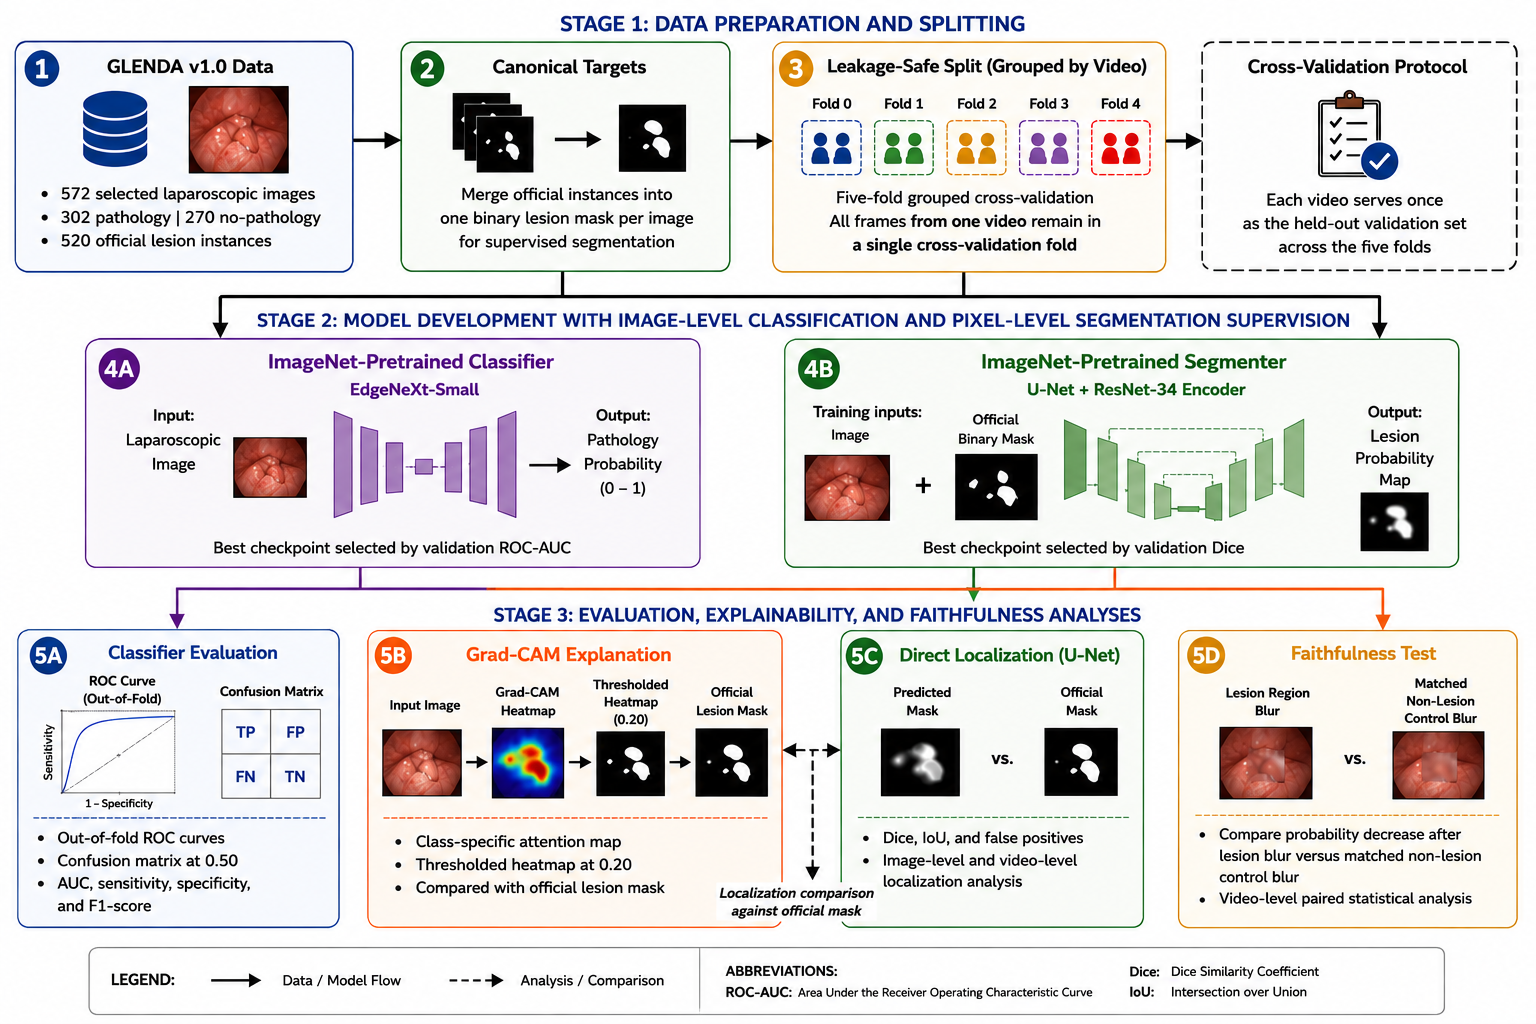
\includegraphics[width=0.96\columnwidth]{figure1_glenda_xai_pipeline.png}
\caption{Overview of the proposed study. The central methodological distinction is between a classifier's post-hoc explanation and a segmentation model trained directly from lesion masks.}
\label{fig:pipeline}
\end{figure}

\subsection{Classifier Model}

The classification model was EdgeNeXt-Small \cite{maaz2022edgenext}, initialized from ImageNet pretrained weights. EdgeNeXt combines convolutional operators with attention-inspired components, allowing local texture features and broader contextual information to be represented efficiently.

Images were resized to $320\times320$ pixels and normalized using ImageNet normalization statistics. The classifier outputs a pathology probability:

\begin{equation}
p_{\text{path}}(x)=P(y=1\mid x),
\end{equation}

where $x$ is an image and $y=1$ denotes pathology.

Training used the fold-specific training partition and was limited to a maximum of 20 epochs. The best model checkpoint was selected by held-out validation ROC-AUC. Early stopping limited additional epochs after no improvement. The primary metric was mean fold-level ROC-AUC. Threshold-dependent metrics were additionally reported at a fixed threshold of 0.50.

\subsection{U-Net Segmentation Model}

The segmentation model was a U-Net \cite{ronneberger2015unet} with a ResNet-34 encoder initialized using ImageNet pretrained weights \cite{he2016resnet}. The encoder extracts hierarchical visual representations; the decoder and skip connections reconstruct a high-resolution lesion probability map.

The segmentation objective combined weighted binary cross-entropy and soft Dice loss:

\begin{equation}
\mathcal{L}_{seg}
=
0.5\mathcal{L}_{WBCE}
+
0.5\mathcal{L}_{Dice}.
\end{equation}

The positive-pixel weight was set to 5.0, reflecting the relative sparsity of lesion pixels. Mild training-only augmentation included horizontal flipping and brightness/contrast variation. U-Net probability maps were thresholded at 0.50 for the reported binary-mask metrics.

\subsection{Evaluation Metrics}

Classifier discrimination was evaluated using ROC-AUC. Accuracy, balanced accuracy, F1-score, sensitivity, specificity, and a confusion matrix were reported at a fixed threshold of 0.50. Because fold models are independently trained and may differ in probability calibration \cite{guo2017calibration}, the average fold-level AUC is emphasized rather than pooled probability calibration.

For binary masks $A$ and $B$, Dice and IoU were defined as:

\begin{equation}
\mathrm{Dice}(A,B)=\frac{2|A\cap B|}{|A|+|B|},
\end{equation}

\begin{equation}
\mathrm{IoU}(A,B)=\frac{|A\cap B|}{|A\cup B|}.
\end{equation}

Positive-image Dice and IoU were computed only on pathology images. For no-pathology images, we reported the false-positive image rate: the fraction of images where the U-Net produced any positive pixel after thresholding.

\section{Explainability and Faithfulness Methodology}

\subsection{Grad-CAM Localization}

Grad-CAM was computed using the held-out classifier corresponding to each image's validation fold. The pathology-class gradient was propagated to the selected convolutional representation to obtain a spatial heatmap \cite{selvaraju2017gradcam}. This heatmap was resized to the image resolution and thresholded at 0.20 to form a binary attention map.

The Grad-CAM threshold was selected in a Fold 0 pilot and held fixed for the remaining folds. This choice is disclosed because thresholding affects overlap values. Grad-CAM results should therefore be interpreted as a transparent fixed-threshold XAI comparison, not as a threshold-free segmentation benchmark.

\subsection{Spatial Alignment with Official Masks}

Grad-CAM Dice and IoU were computed against the same official masks used to train and evaluate U-Net. Scores were calculated per pathology image and then averaged per pathology video. Video-level averaging reduces the risk that multiple highly correlated frames from one recording dominate the analysis.

This comparison directly tests whether a classifier explanation is spatially as informative as a segmentation model trained on pixel-level supervision. A superior U-Net score would not imply that Grad-CAM is clinically useless; rather, it would indicate that the post-hoc explanation is coarser than a dedicated delineation model.

\subsection{Counterfactual Faithfulness Test}

Spatial overlap does not establish that a classifier actually depends on the highlighted lesion. To test functional dependence, all 302 held-out pathology images underwent three evaluations: the original image, an image with official lesion pixels Gaussian-blurred, and an image with a matched lesion-shaped non-lesion control region Gaussian-blurred.

The control region was generated by translating the lesion shape to a minimally overlapping non-lesion position where possible. This is stronger than simply blurring a random region because it approximately matches intervention area and shape.

For perturbation region $r$, probability drop was:

\begin{equation}
\Delta_r =
p_{\text{path}}(x)
-
p_{\text{path}}(x_r).
\end{equation}

The faithfulness difference was:

\begin{equation}
F=
\Delta_{\text{lesion}}
-
\Delta_{\text{control}}.
\end{equation}

A positive $F$ indicates that lesion perturbation reduced pathology confidence more than control perturbation. Results were aggregated across 168 held-out pathology videos. A one-sided paired Wilcoxon signed-rank test \cite{wilcoxon1945} and a 5,000-resample bootstrap confidence interval were applied to the video-level differences.

\subsection{Interpretation of XAI Evidence}

This study uses three complementary types of explanation evidence: \textbf{visual evidence}, provided by Grad-CAM heatmaps and prediction overlays; \textbf{spatial evidence}, quantified through Dice and IoU overlap with official lesion masks; and \textbf{functional evidence}, measured through probability change after lesion-region versus control-region perturbation.

This layered evaluation is more rigorous than visual heatmaps alone. Still, it does not prove causal medical reasoning, fully eliminate background reliance, or establish clinical usefulness. It supports the narrower conclusion that lesion-region information is meaningfully associated with classifier confidence in this dataset.

\section{Results}

\subsection{Cross-Validated Classifier and Segmentation Performance}

Table~\ref{tab:foldresults} summarizes results across five held-out folds. The EdgeNeXt-Small classifier achieved mean fold-level ROC-AUC of $0.9652\pm0.0113$. The fold-level AUC values were consistently high, ranging from 0.9502 to 0.9817.

The U-Net achieved mean positive-image Dice of $0.4377\pm0.0492$ and mean IoU of $0.3166\pm0.0402$. The variation across folds reflects the diversity of lesion visibility and boundary quality. The U-Net negative-image false-positive rate was 0.4793 at threshold 0.50, showing that direct segmentation remains imperfect and requires expert review.

\begin{table*}[t]
\caption{Held-out five-fold performance. U-Net metrics use a fixed 0.50 probability threshold.}
\label{tab:foldresults}
\centering
\resizebox{\textwidth}{!}{
\begin{tabular}{c c c c c c c c}
\toprule
Fold & Classifier AUC & Balanced accuracy & Classifier F1 & U-Net mean Dice & U-Net median Dice & U-Net mean IoU & U-Net negative FP rate \\
\midrule
0 & 0.9623 & 0.8962 & 0.9134 & 0.5001 & 0.5633 & 0.3666 & 0.7000 \\
1 & 0.9817 & 0.9596 & 0.9592 & 0.4397 & 0.4899 & 0.3143 & 0.3400 \\
2 & 0.9675 & 0.6857 & 0.7250 & 0.3629 & 0.3526 & 0.2550 & 0.5000 \\
3 & 0.9641 & 0.9068 & 0.9048 & 0.4349 & 0.5033 & 0.3179 & 0.3167 \\
4 & 0.9502 & 0.8762 & 0.8923 & 0.4510 & 0.4763 & 0.3293 & 0.5400 \\
\midrule
Mean & 0.9652 & 0.8649 & 0.8789 & 0.4377 & 0.4771 & 0.3166 & 0.4793 \\
Standard deviation & 0.0113 & 0.1048 & 0.0897 & 0.0492 & 0.0771 & 0.0402 & 0.1571 \\
\bottomrule
\end{tabular}}
\end{table*}

\begin{figure}[t]
\centering
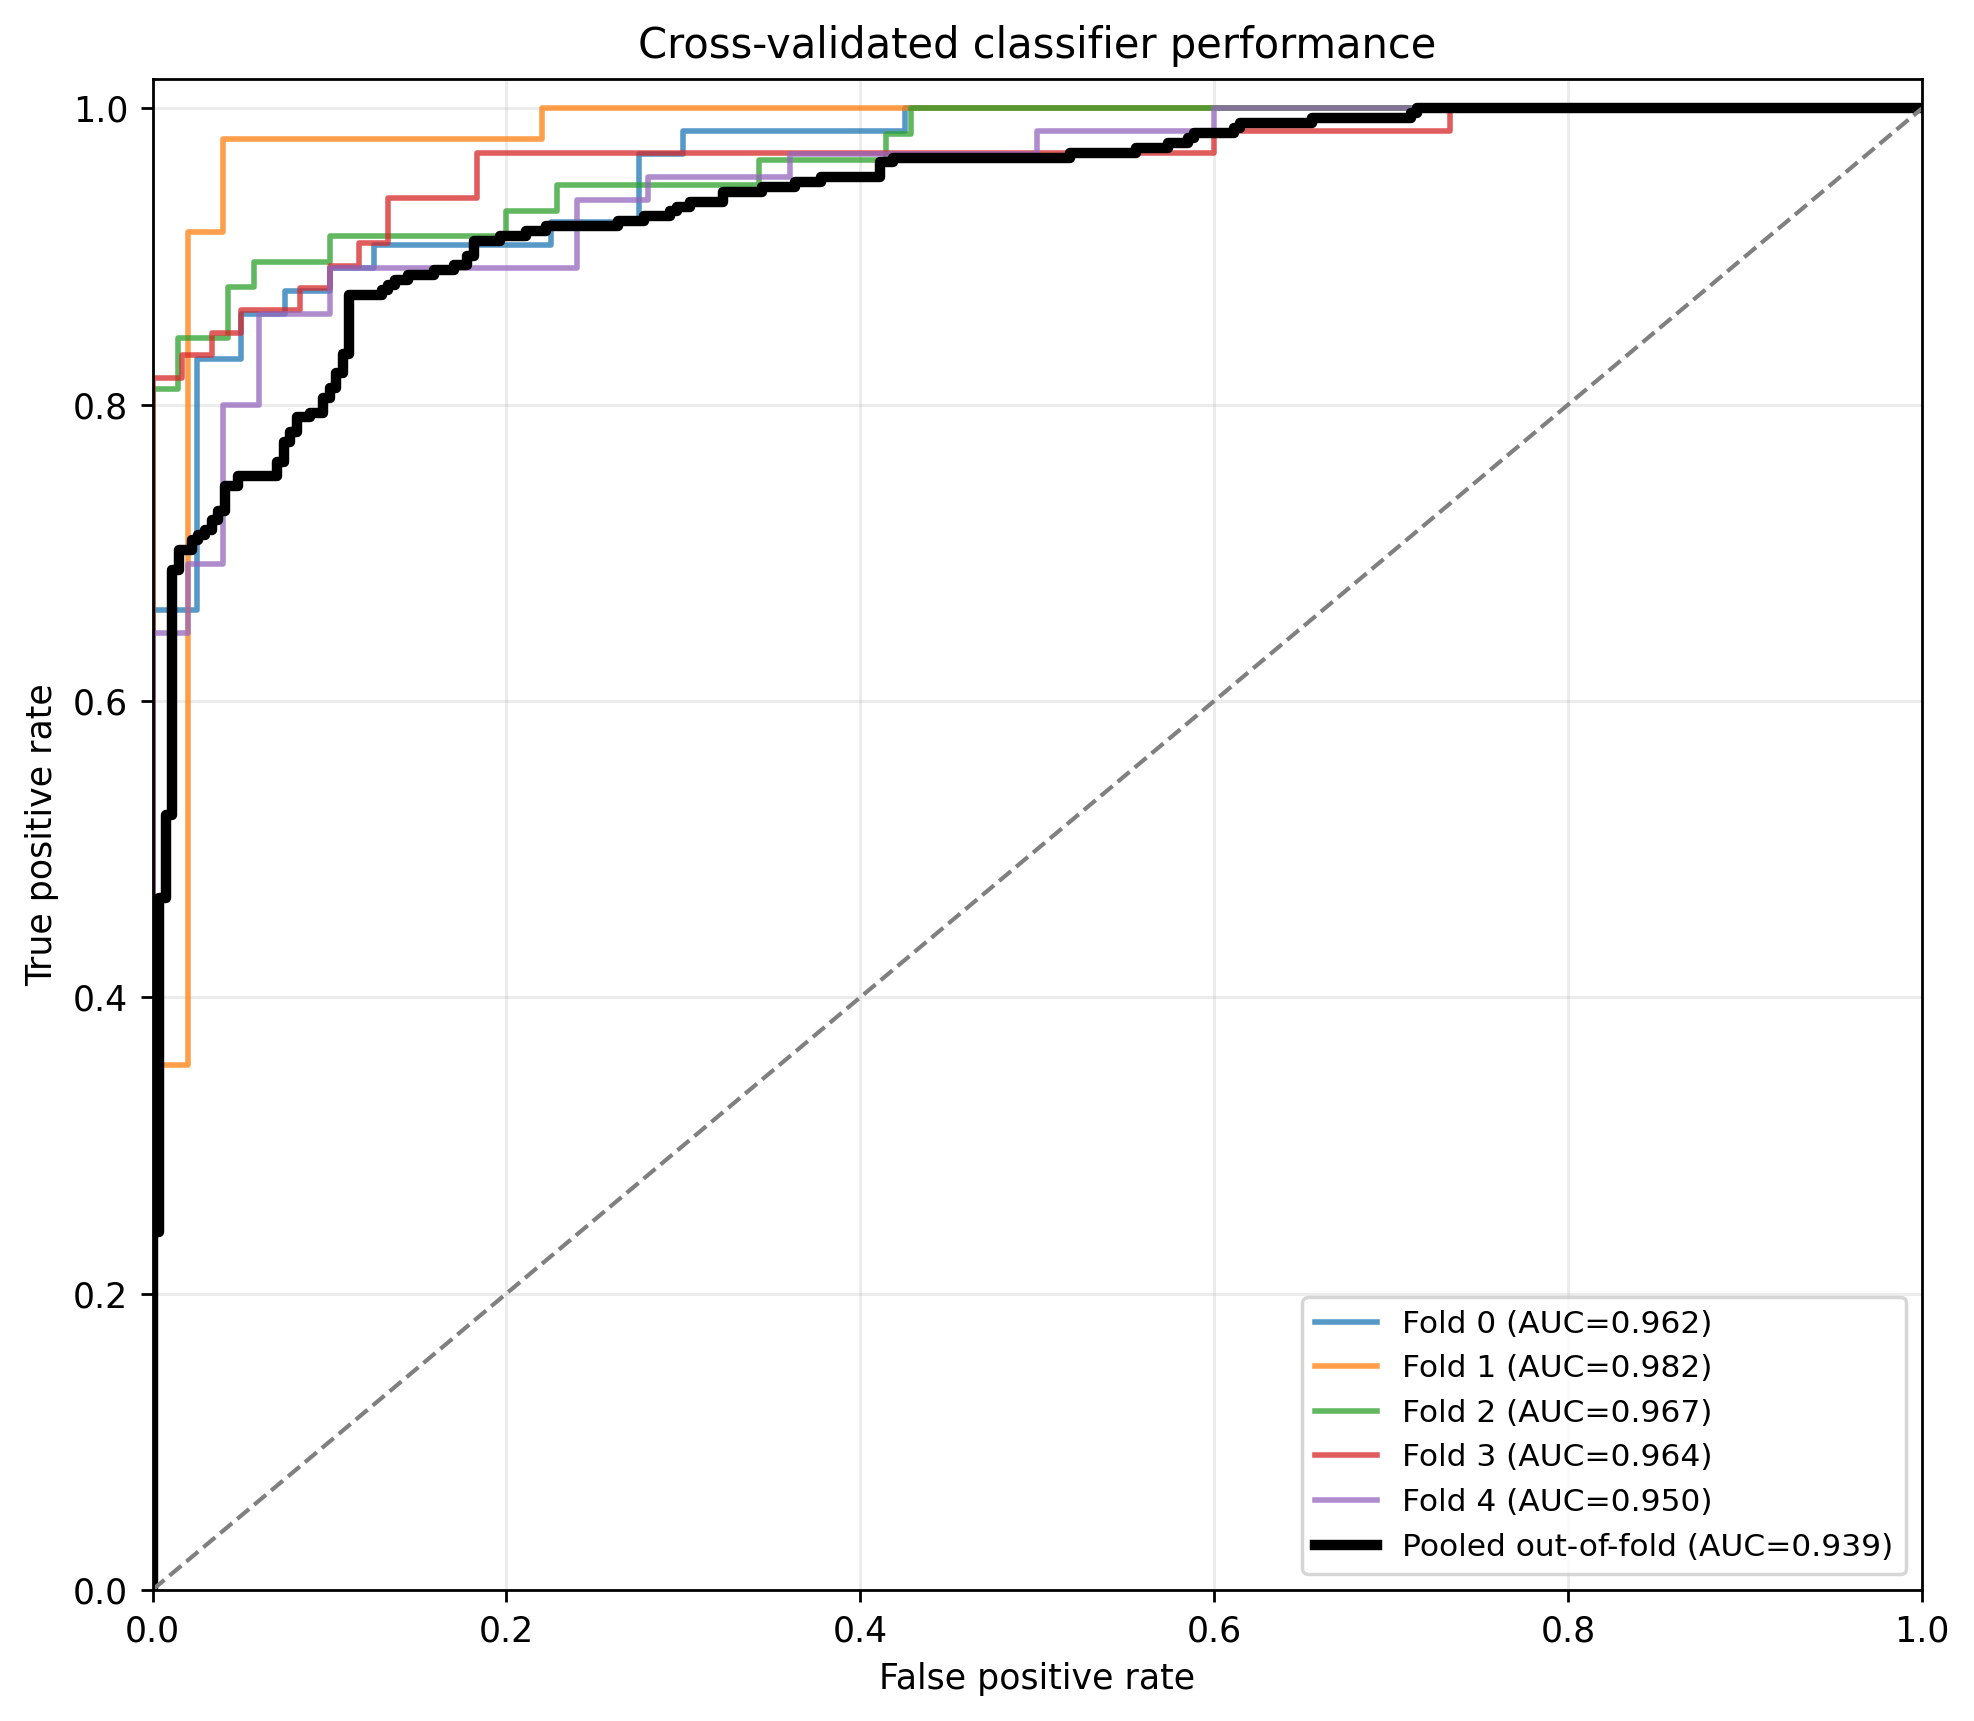
\includegraphics[width=0.96\columnwidth]{figure_classifier_cross_validated_roc.png}
\caption{Classifier ROC curves across the five held-out folds. The consistently elevated curves demonstrate strong ranking performance under video-level separation.}
\label{fig:roc}
\end{figure}

\begin{figure}[t]
\centering
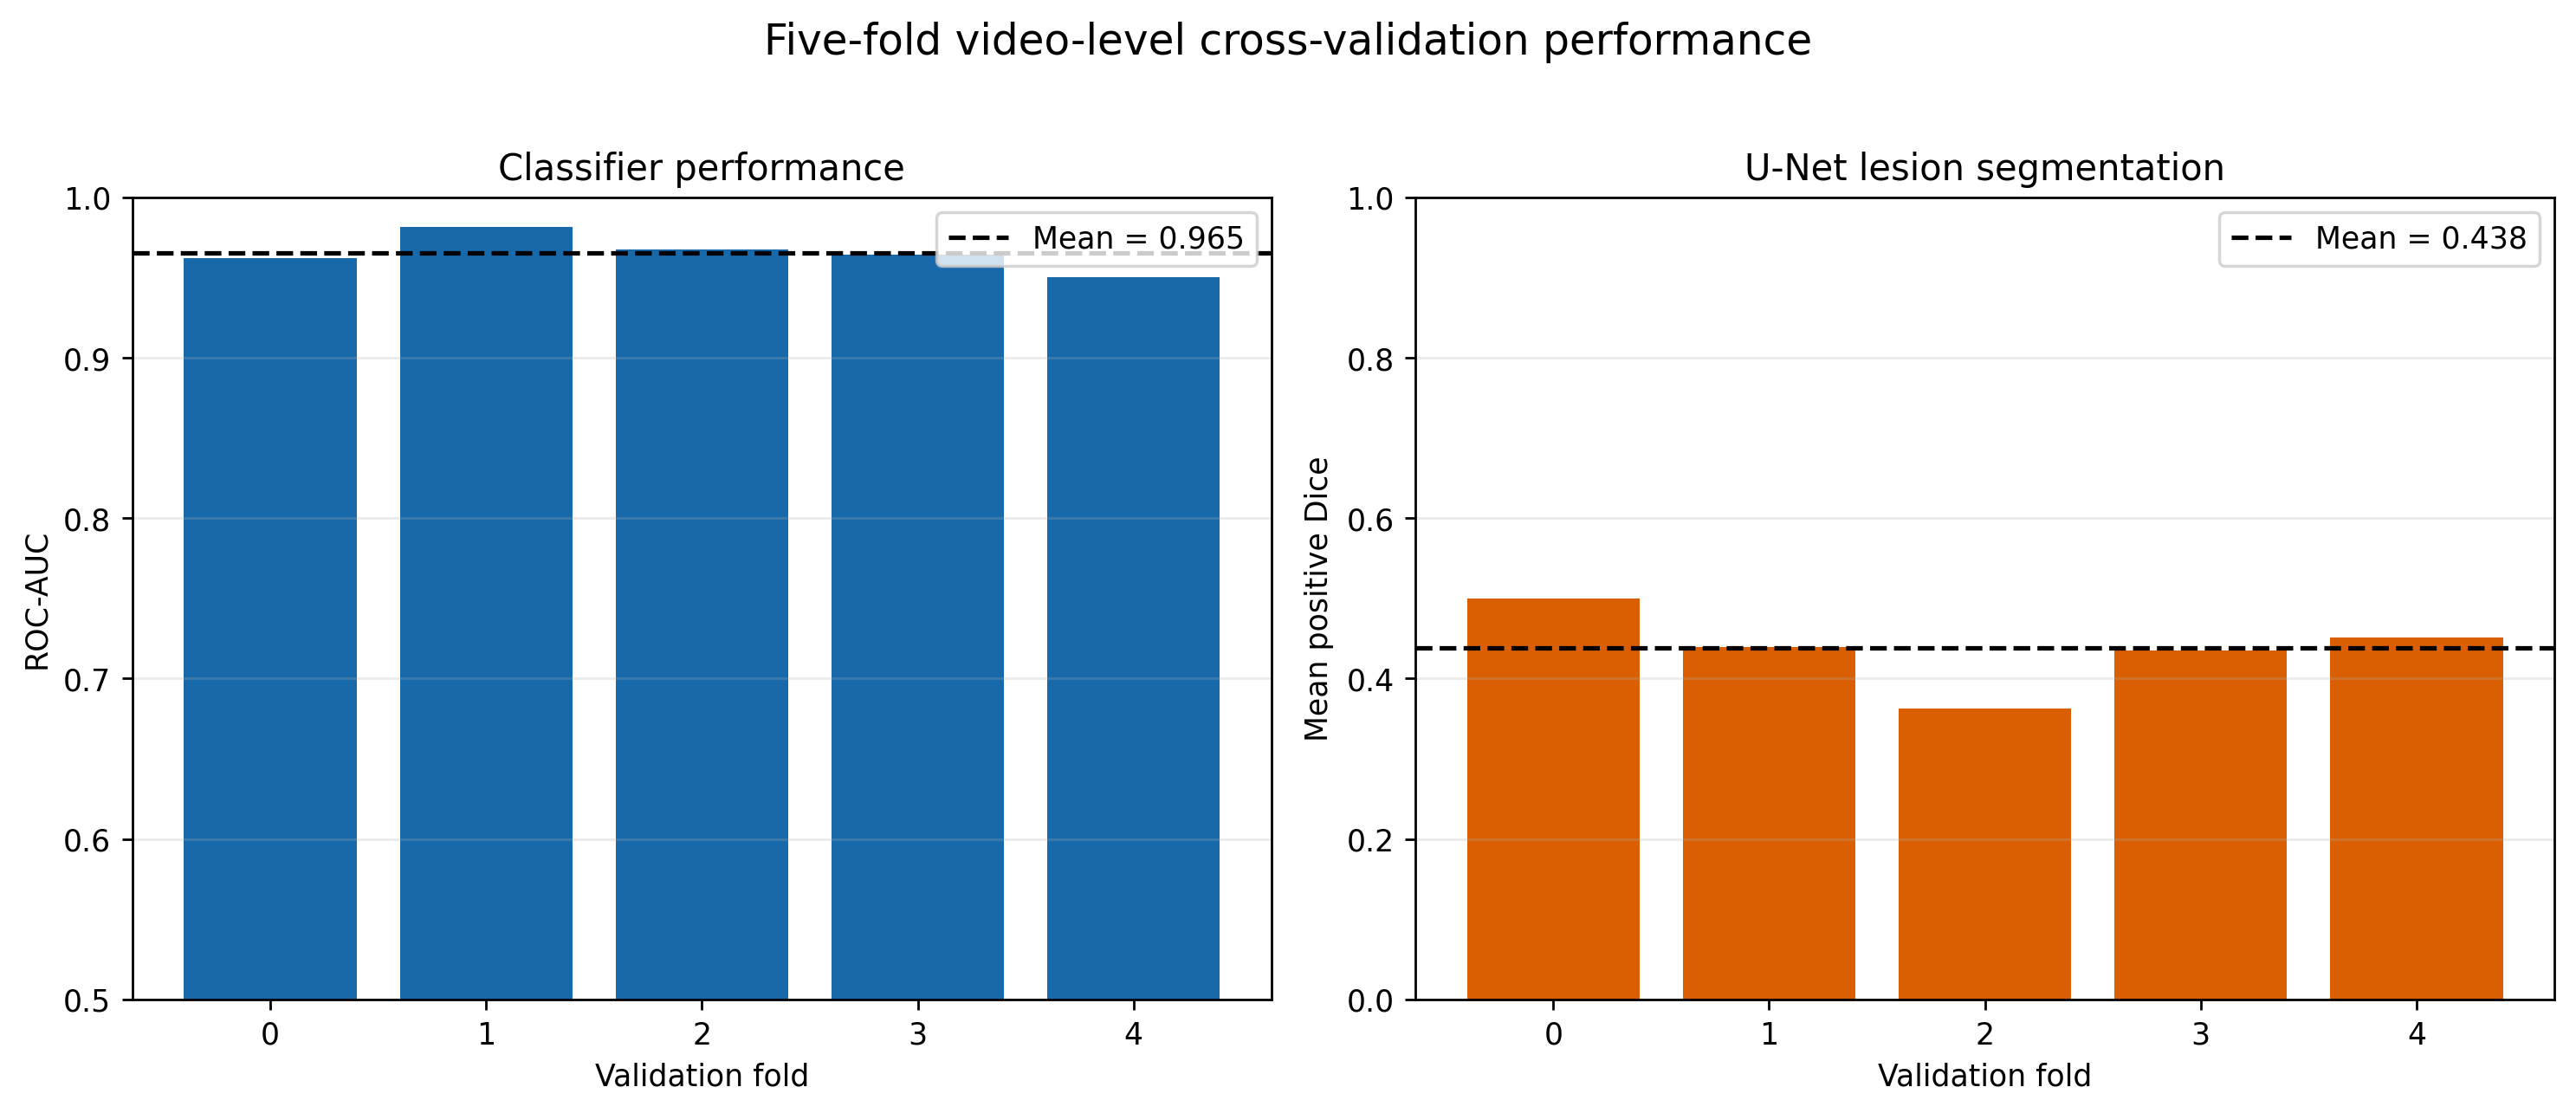
\includegraphics[width=0.96\columnwidth]{figure_foldwise_model_performance.png}
\caption{Fold-wise performance comparison. Classifier discrimination is consistently high, whereas segmentation overlap varies more due to heterogeneous lesion appearance and difficult boundaries.}
\label{fig:foldperformance}
\end{figure}

\subsection{Out-of-Fold Confusion Matrix}

The pooled out-of-fold confusion matrix contains one prediction for every image, generated only by the model that did not train on its video's frames. At threshold 0.50, the classifier produced 278 true positives, 209 true negatives, 24 false negatives, and 61 false positives. Sensitivity was 0.921, specificity was 0.774, and accuracy was 0.851.

The greater sensitivity than specificity suggests that the chosen threshold favors flagging pathology over rejecting no-pathology images. This may be desirable for an exploratory review tool but also increases false-alert burden. Therefore, the confusion matrix should be interpreted alongside ROC-AUC, not as proof of a final clinical operating threshold.

\begin{figure}[t]
\centering
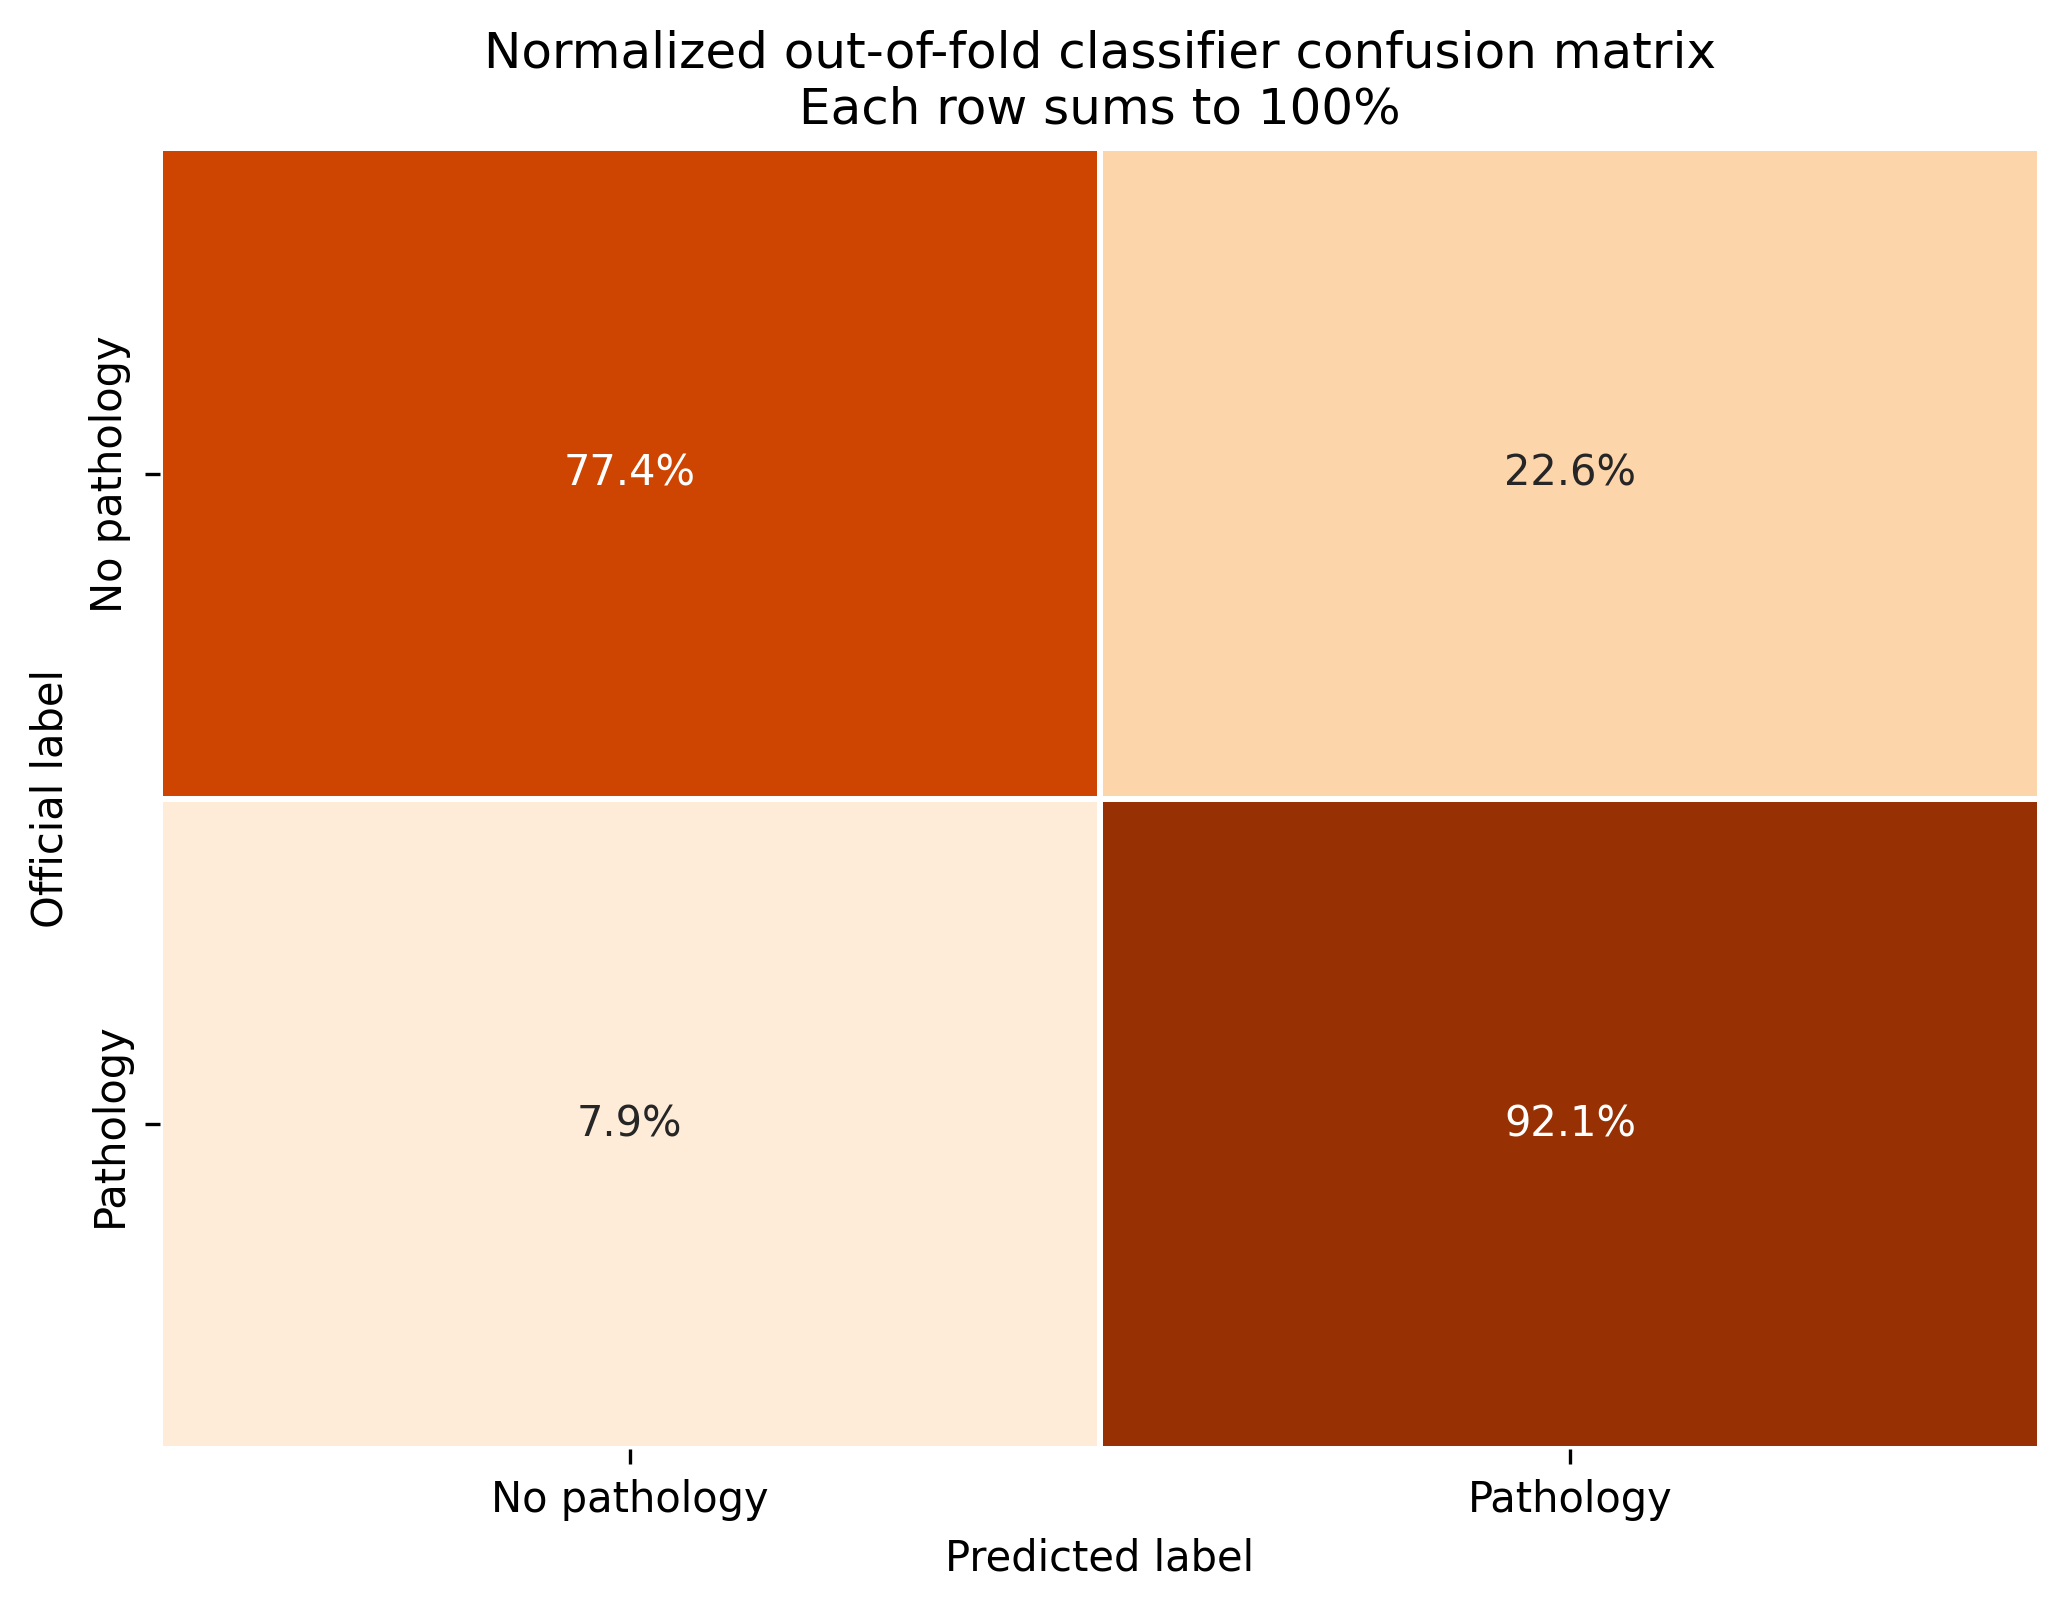
\includegraphics[width=0.96\columnwidth]{figure_classifier_confusion_matrix_normalized.png}
\caption{Normalized out-of-fold confusion matrix at the fixed pathology threshold of 0.50. The figure makes the sensitivity-specificity trade-off transparent.}
\label{fig:confusion}
\end{figure}

\subsection{Distribution of Segmentation Accuracy}

The U-Net mean Dice does not fully describe the range of image-level outcomes. Some held-out pathology images achieved high overlap, while others had low or zero Dice. This variation is expected because lesions differ in extent, color, local anatomy, instrument interference, and annotation clarity.

Figure~\ref{fig:dicedistribution} should display boxplots and individual points for all positive-image Dice scores across folds. It is important for the paper because it avoids reporting only a favorable average. A model with moderate mean Dice can still be useful for some lesion appearances while failing on others.

\begin{figure}[t]
\centering
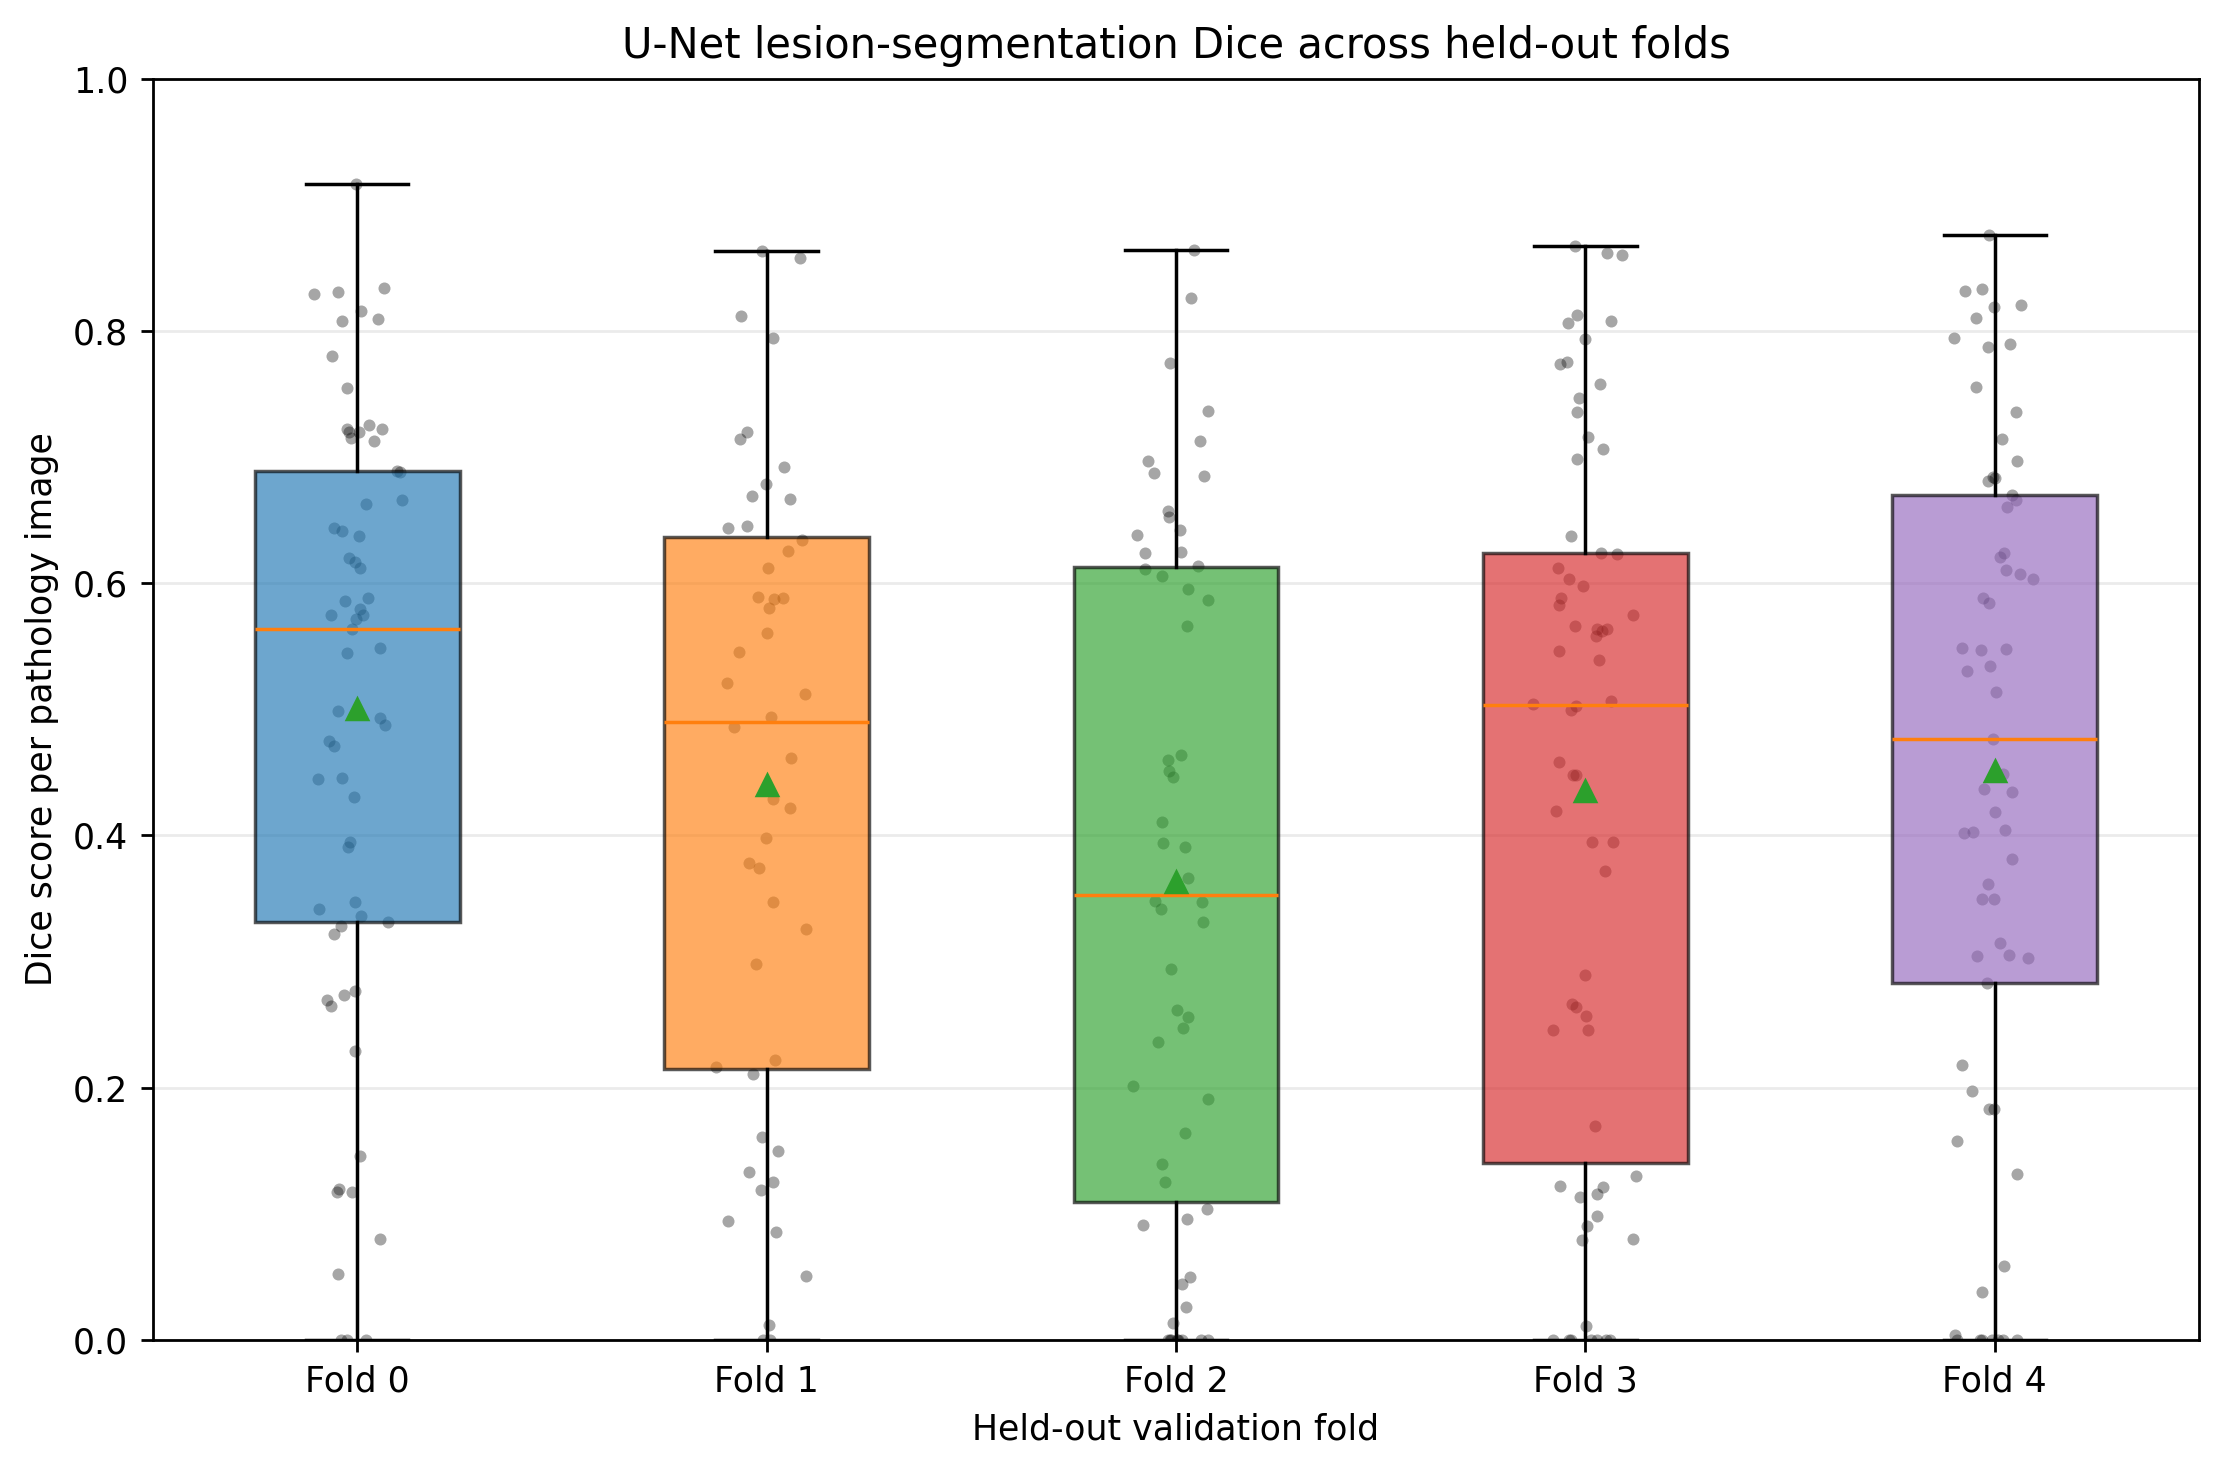
\includegraphics[width=0.96\columnwidth]{figure_unet_dice_distribution_by_fold.png}
\caption{Distribution of U-Net Dice across pathology images. Wide within-fold variation indicates that localization performance depends strongly on individual lesion appearance and image conditions.}
\label{fig:dicedistribution}
\end{figure}

\subsection{U-Net versus Grad-CAM Localization}

Table~\ref{tab:localization} compares direct U-Net segmentation with post-hoc Grad-CAM localization. At image level, U-Net mean Dice was 0.439, while Grad-CAM mean Dice was 0.249. At video level, U-Net mean Dice was 0.459, compared with 0.274 for Grad-CAM. The mean video-level difference was 0.185 in favor of U-Net.

U-Net achieved higher mean localization Dice in 136 of 168 pathology videos. Grad-CAM achieved higher Dice in 32 videos. This result shows a general advantage of direct pixel supervision, while preserving the important observation that post-hoc attention can sometimes better overlap the official lesion in individual cases.

\begin{table}[t]
\caption{Localization comparison using official lesion masks.}
\label{tab:localization}
\centering
\begin{tabular}{l c c c}
\toprule
Unit & $n$ & U-Net Dice & Grad-CAM Dice \\
\midrule
Pathology images & 302 & 0.439 & 0.249 \\
Pathology videos & 168 & 0.459 & 0.274 \\
\bottomrule
\end{tabular}
\end{table}

\begin{figure}[t]
\centering
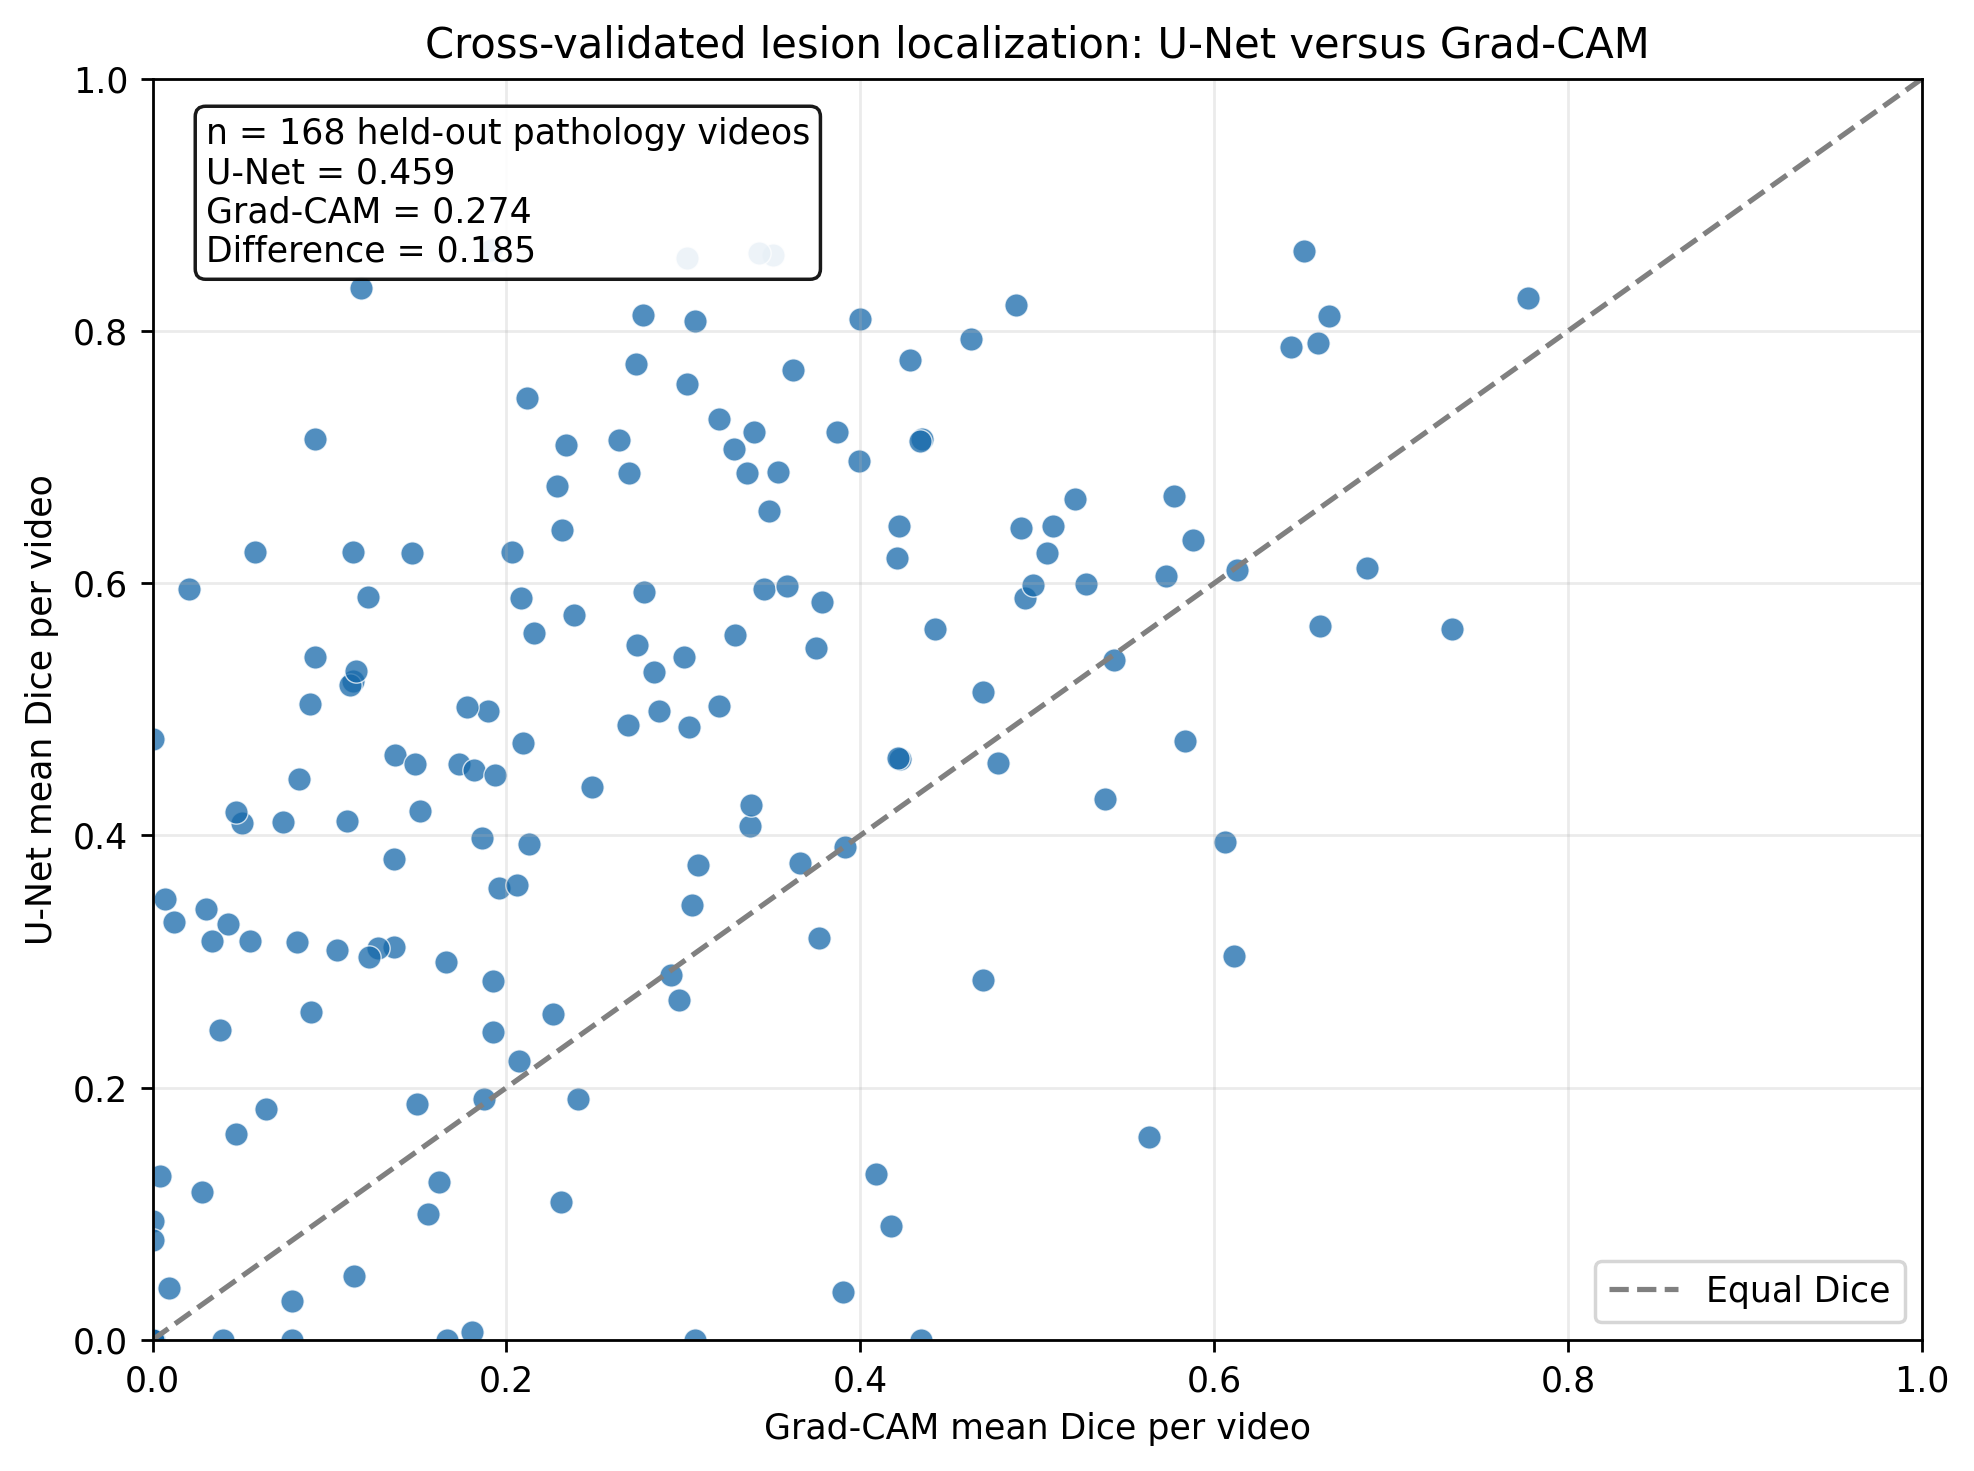
\includegraphics[width=0.96\columnwidth]{figure_video_level_unet_vs_gradcam_scatter.png}
\caption{Video-level comparison of direct segmentation and Grad-CAM localization. Most points above the diagonal indicate more accurate U-Net overlap with official lesion masks.}
\label{fig:scatter}
\end{figure}

\begin{figure}[t]
\centering
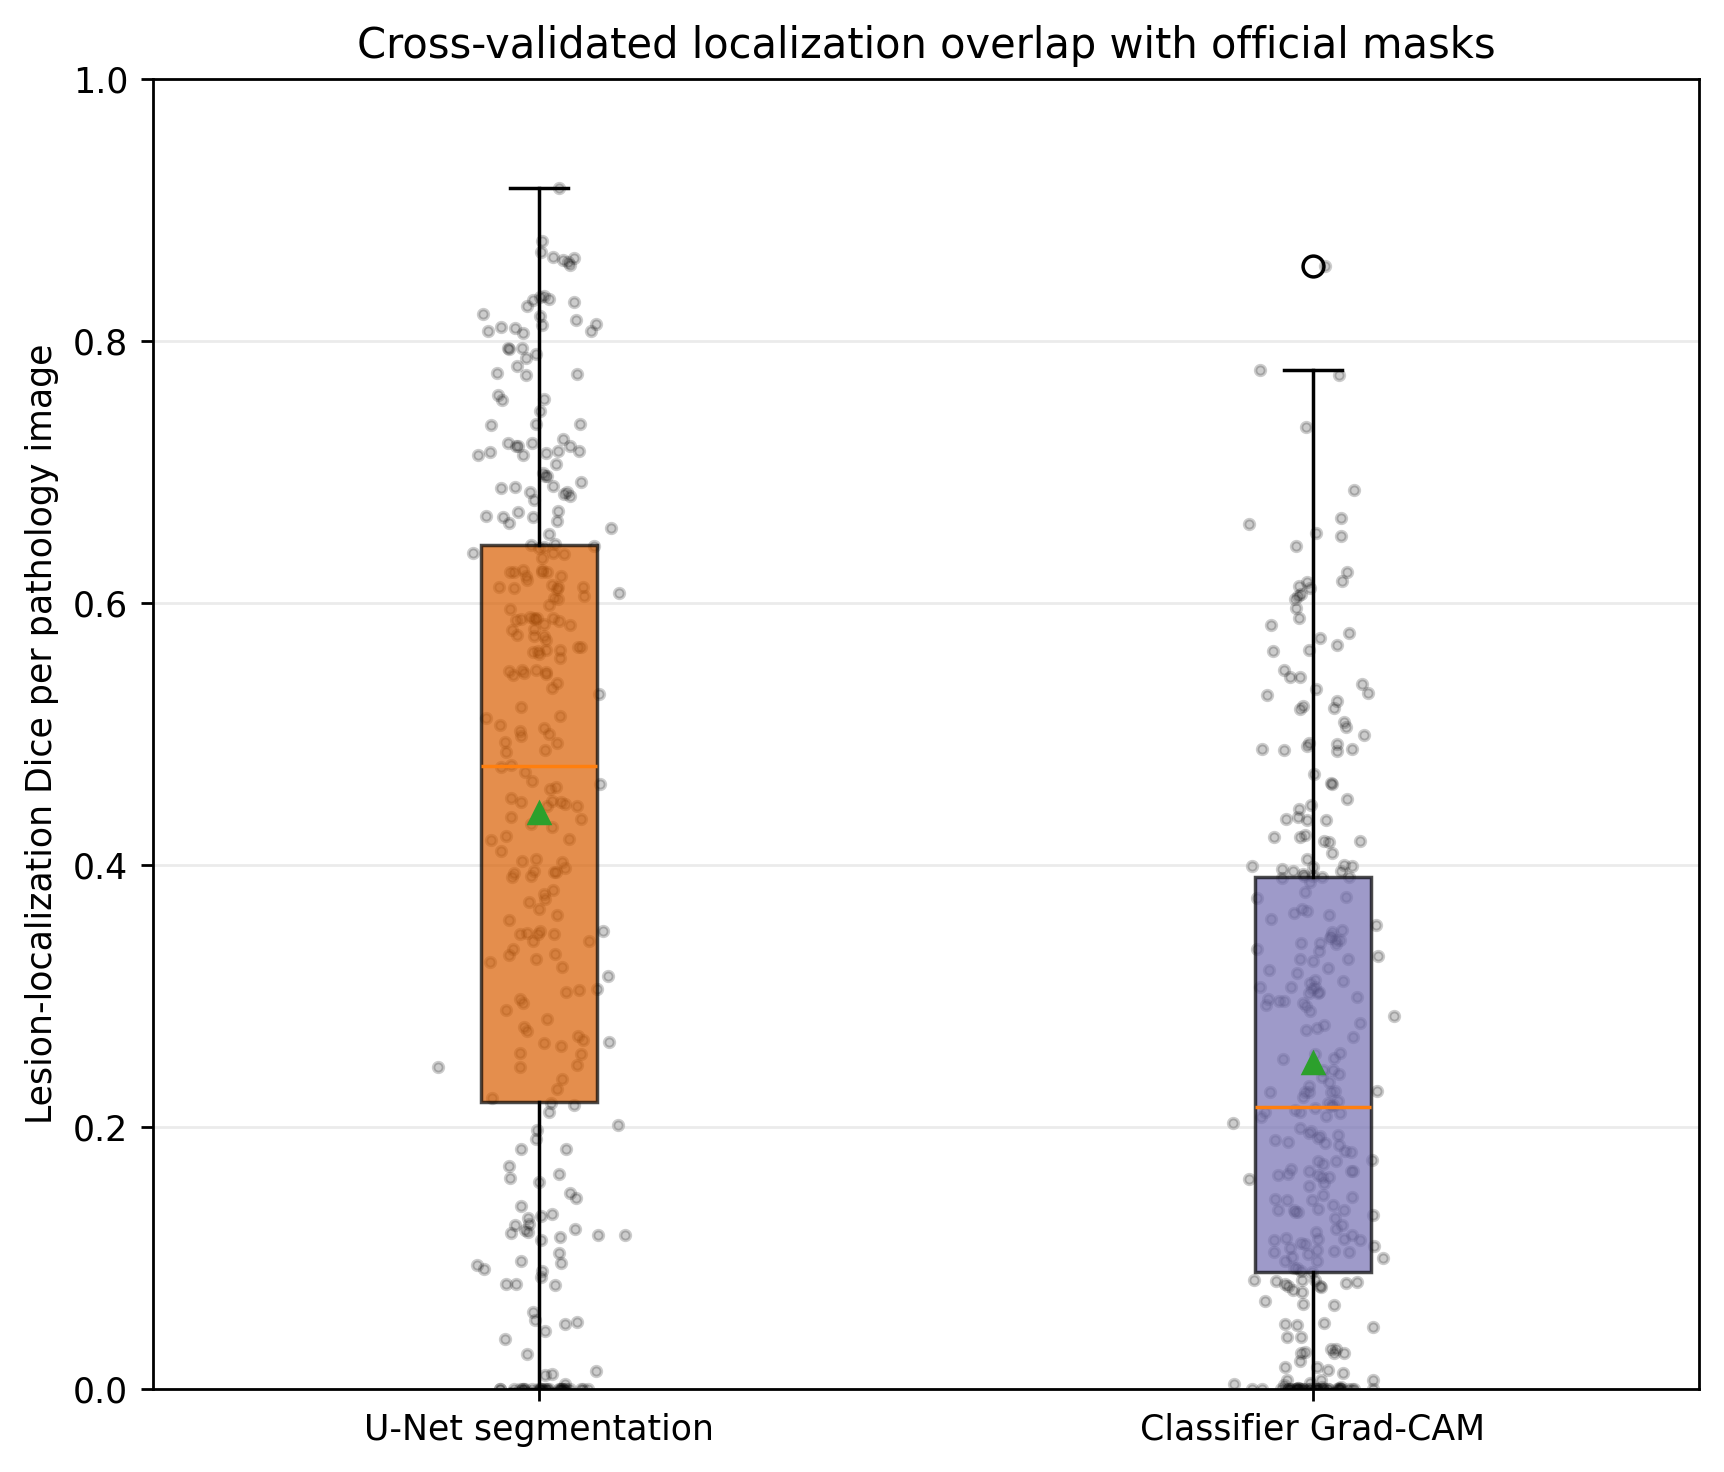
\includegraphics[width=0.96\columnwidth]{figure_image_level_unet_vs_gradcam_distribution.png}
\caption{Image-level distribution of localization Dice. U-Net has higher central overlap, while the figure also demonstrates substantial image-specific variability for both methods.}
\label{fig:localizationdistribution}
\end{figure}

\subsection{Qualitative Examples}

The paper includes representative examples instead of only numerical summaries. The selected cases show a best U-Net localization case, a case with a large U-Net advantage, a case where both methods localize well, a typical held-out pathology case, a counterexample where Grad-CAM outperforms U-Net, and a difficult case where both methods fail.

This figure is important for credibility. A useful medical AI paper should not show only visually successful predictions. Failure cases illustrate why the current system requires clinician review and why future work must improve robustness.

\begin{figure}[t]
\centering
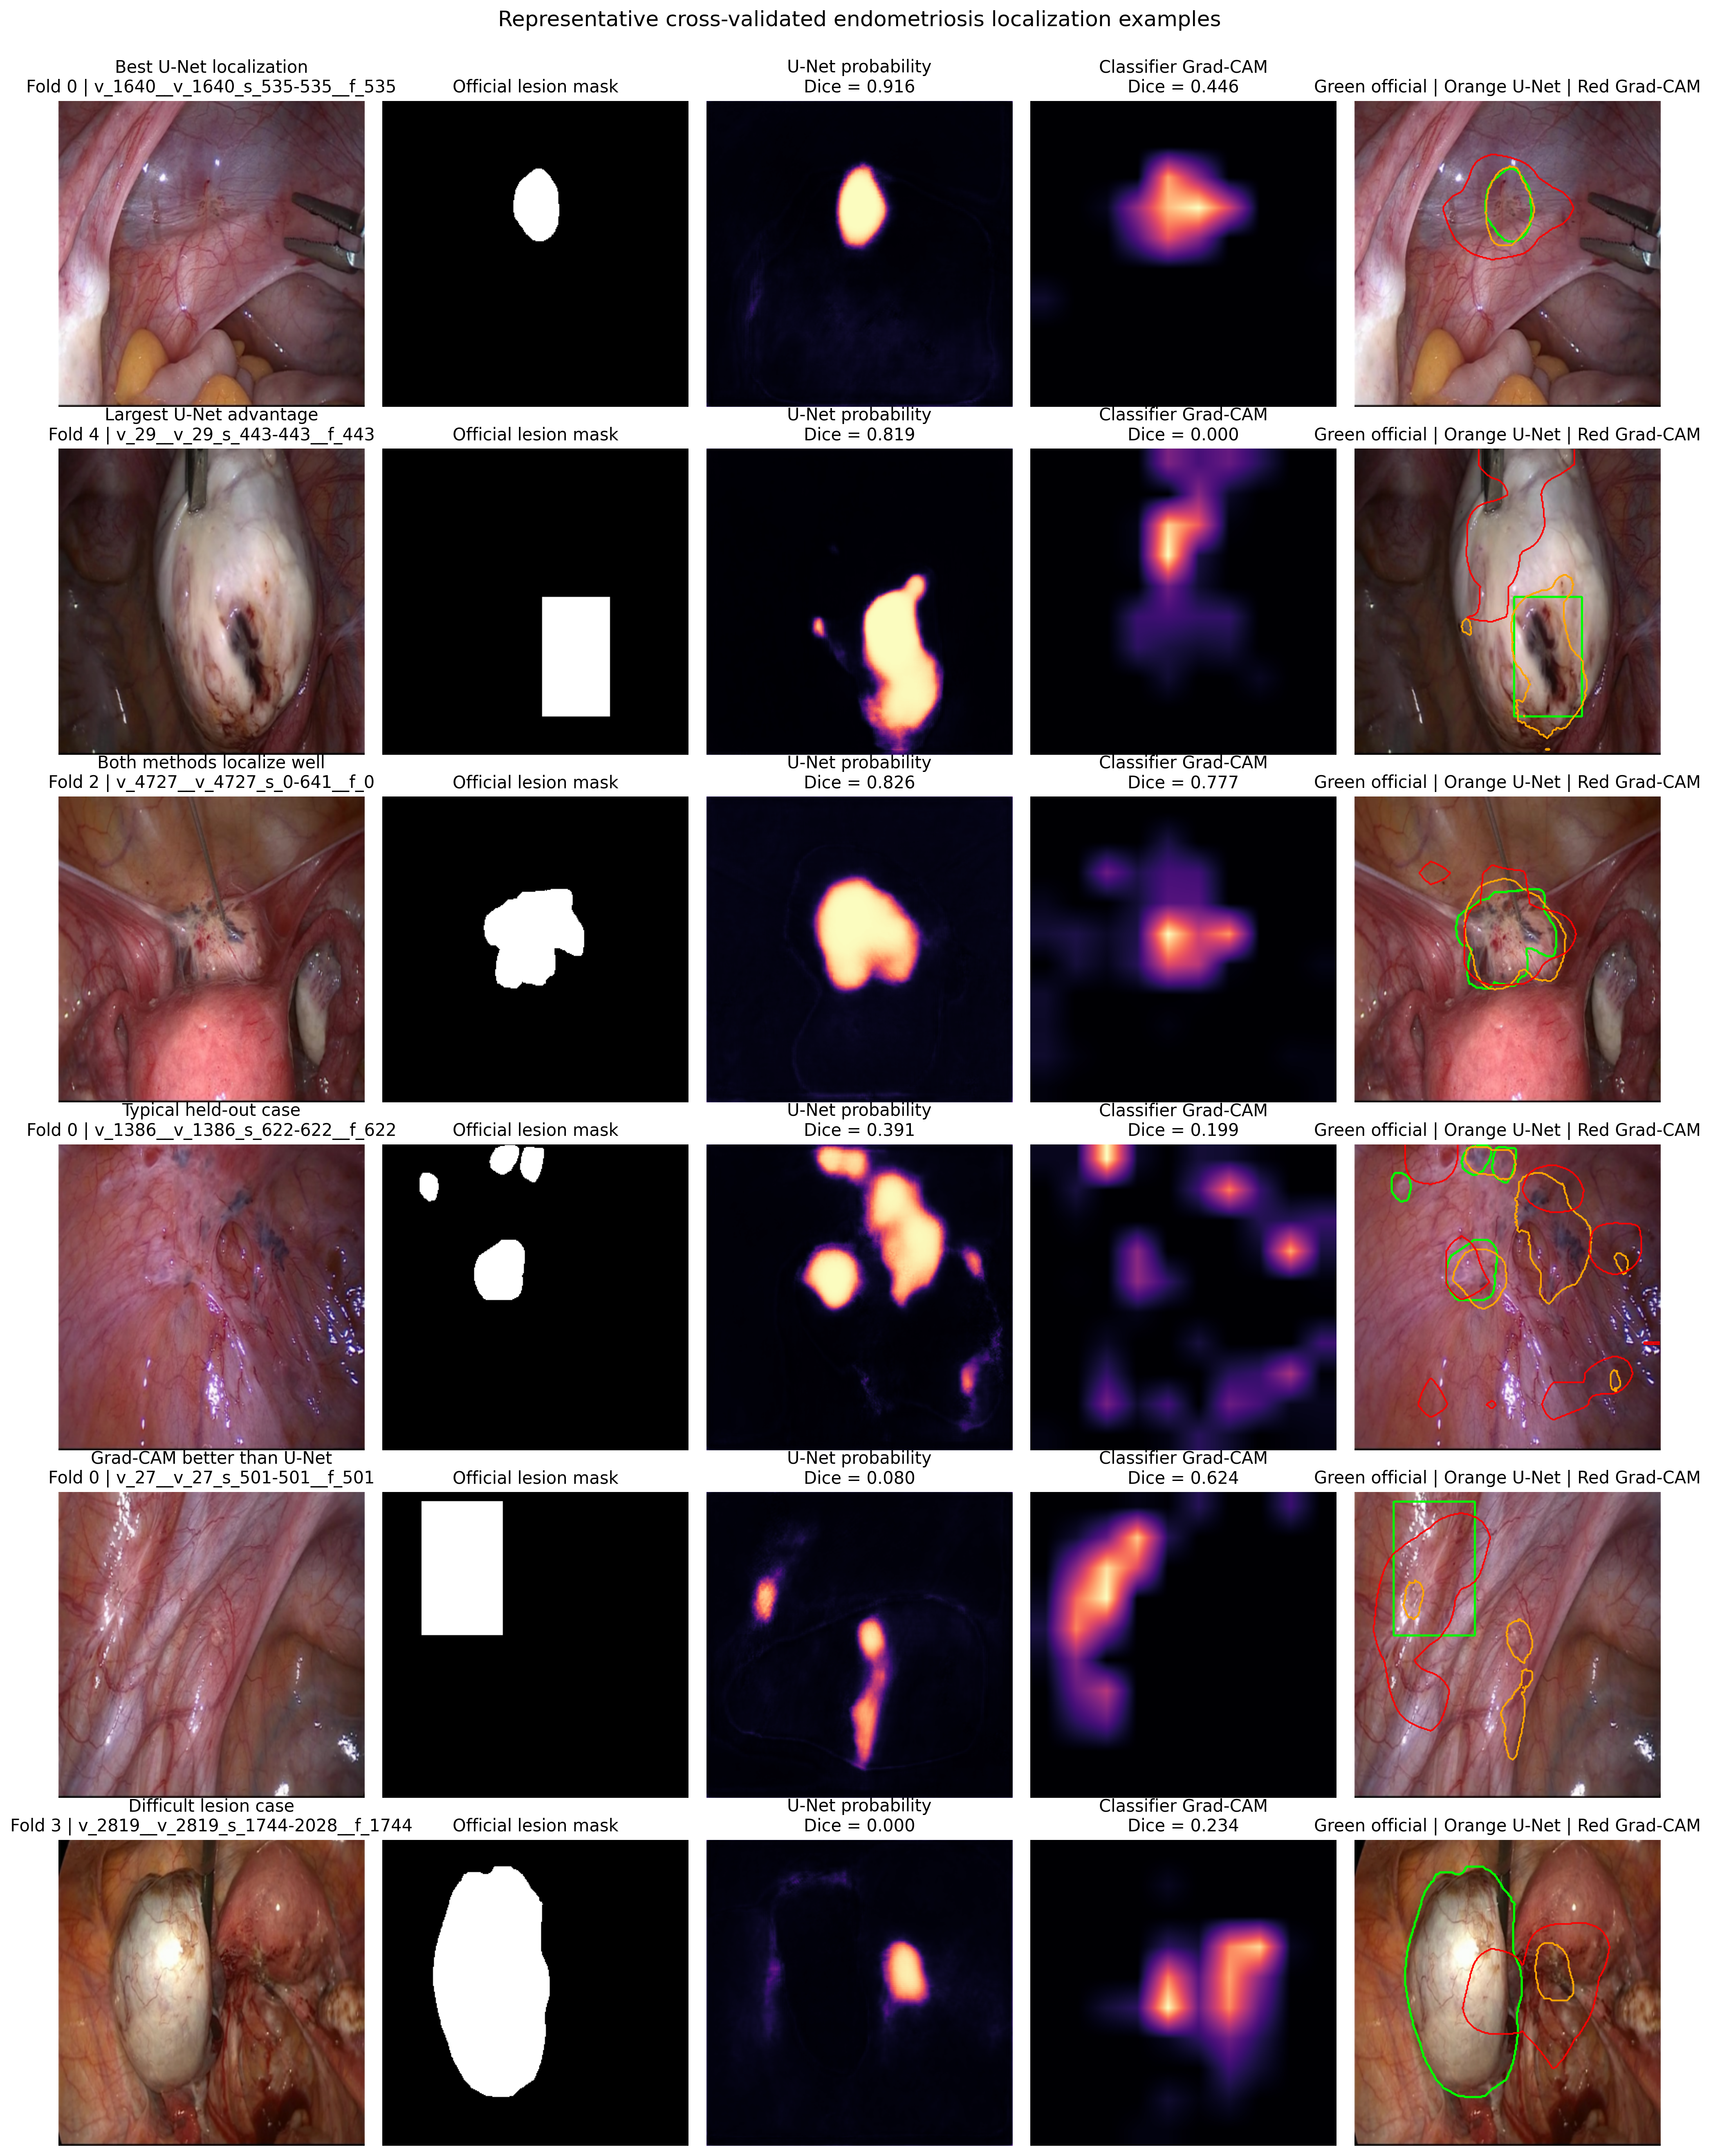
\includegraphics[width=0.75\columnwidth]{figure_qualitative_unet_vs_gradcam_examples.png}
\caption{Representative cross-validated localization examples, including successful, typical, counterexample, and difficult cases. This balanced presentation shows that U-Net generally provides tighter localization but that neither model is clinically sufficient on every image.}
\label{fig:qualitative}
\end{figure}

\subsection{Counterfactual Faithfulness Results}

The counterfactual test provides functional evidence that the classifier depends more strongly on lesion information than on matched control information. Across 168 held-out pathology videos, blurring the official lesion region reduced pathology probability by 0.1516 on average. Blurring the matched non-lesion control region reduced probability by only 0.0007. The mean paired difference was 0.1508.

The bootstrap 95\% confidence interval for the mean video-level difference was [0.1129, 0.1927]. The one-sided paired Wilcoxon test gave $p=2.719\times10^{-23}$. This supports the conclusion that lesion-region perturbation has a substantially larger effect on classifier confidence than a similarly shaped non-lesion perturbation.

The result should still be interpreted cautiously. Gaussian blurring is an artificial image manipulation; it does not prove that the classifier has learned human-style diagnostic reasoning. It does, however, provide stronger evidence than a heatmap alone that lesion pixels contribute meaningfully to the output.

\begin{figure}[t]
\centering
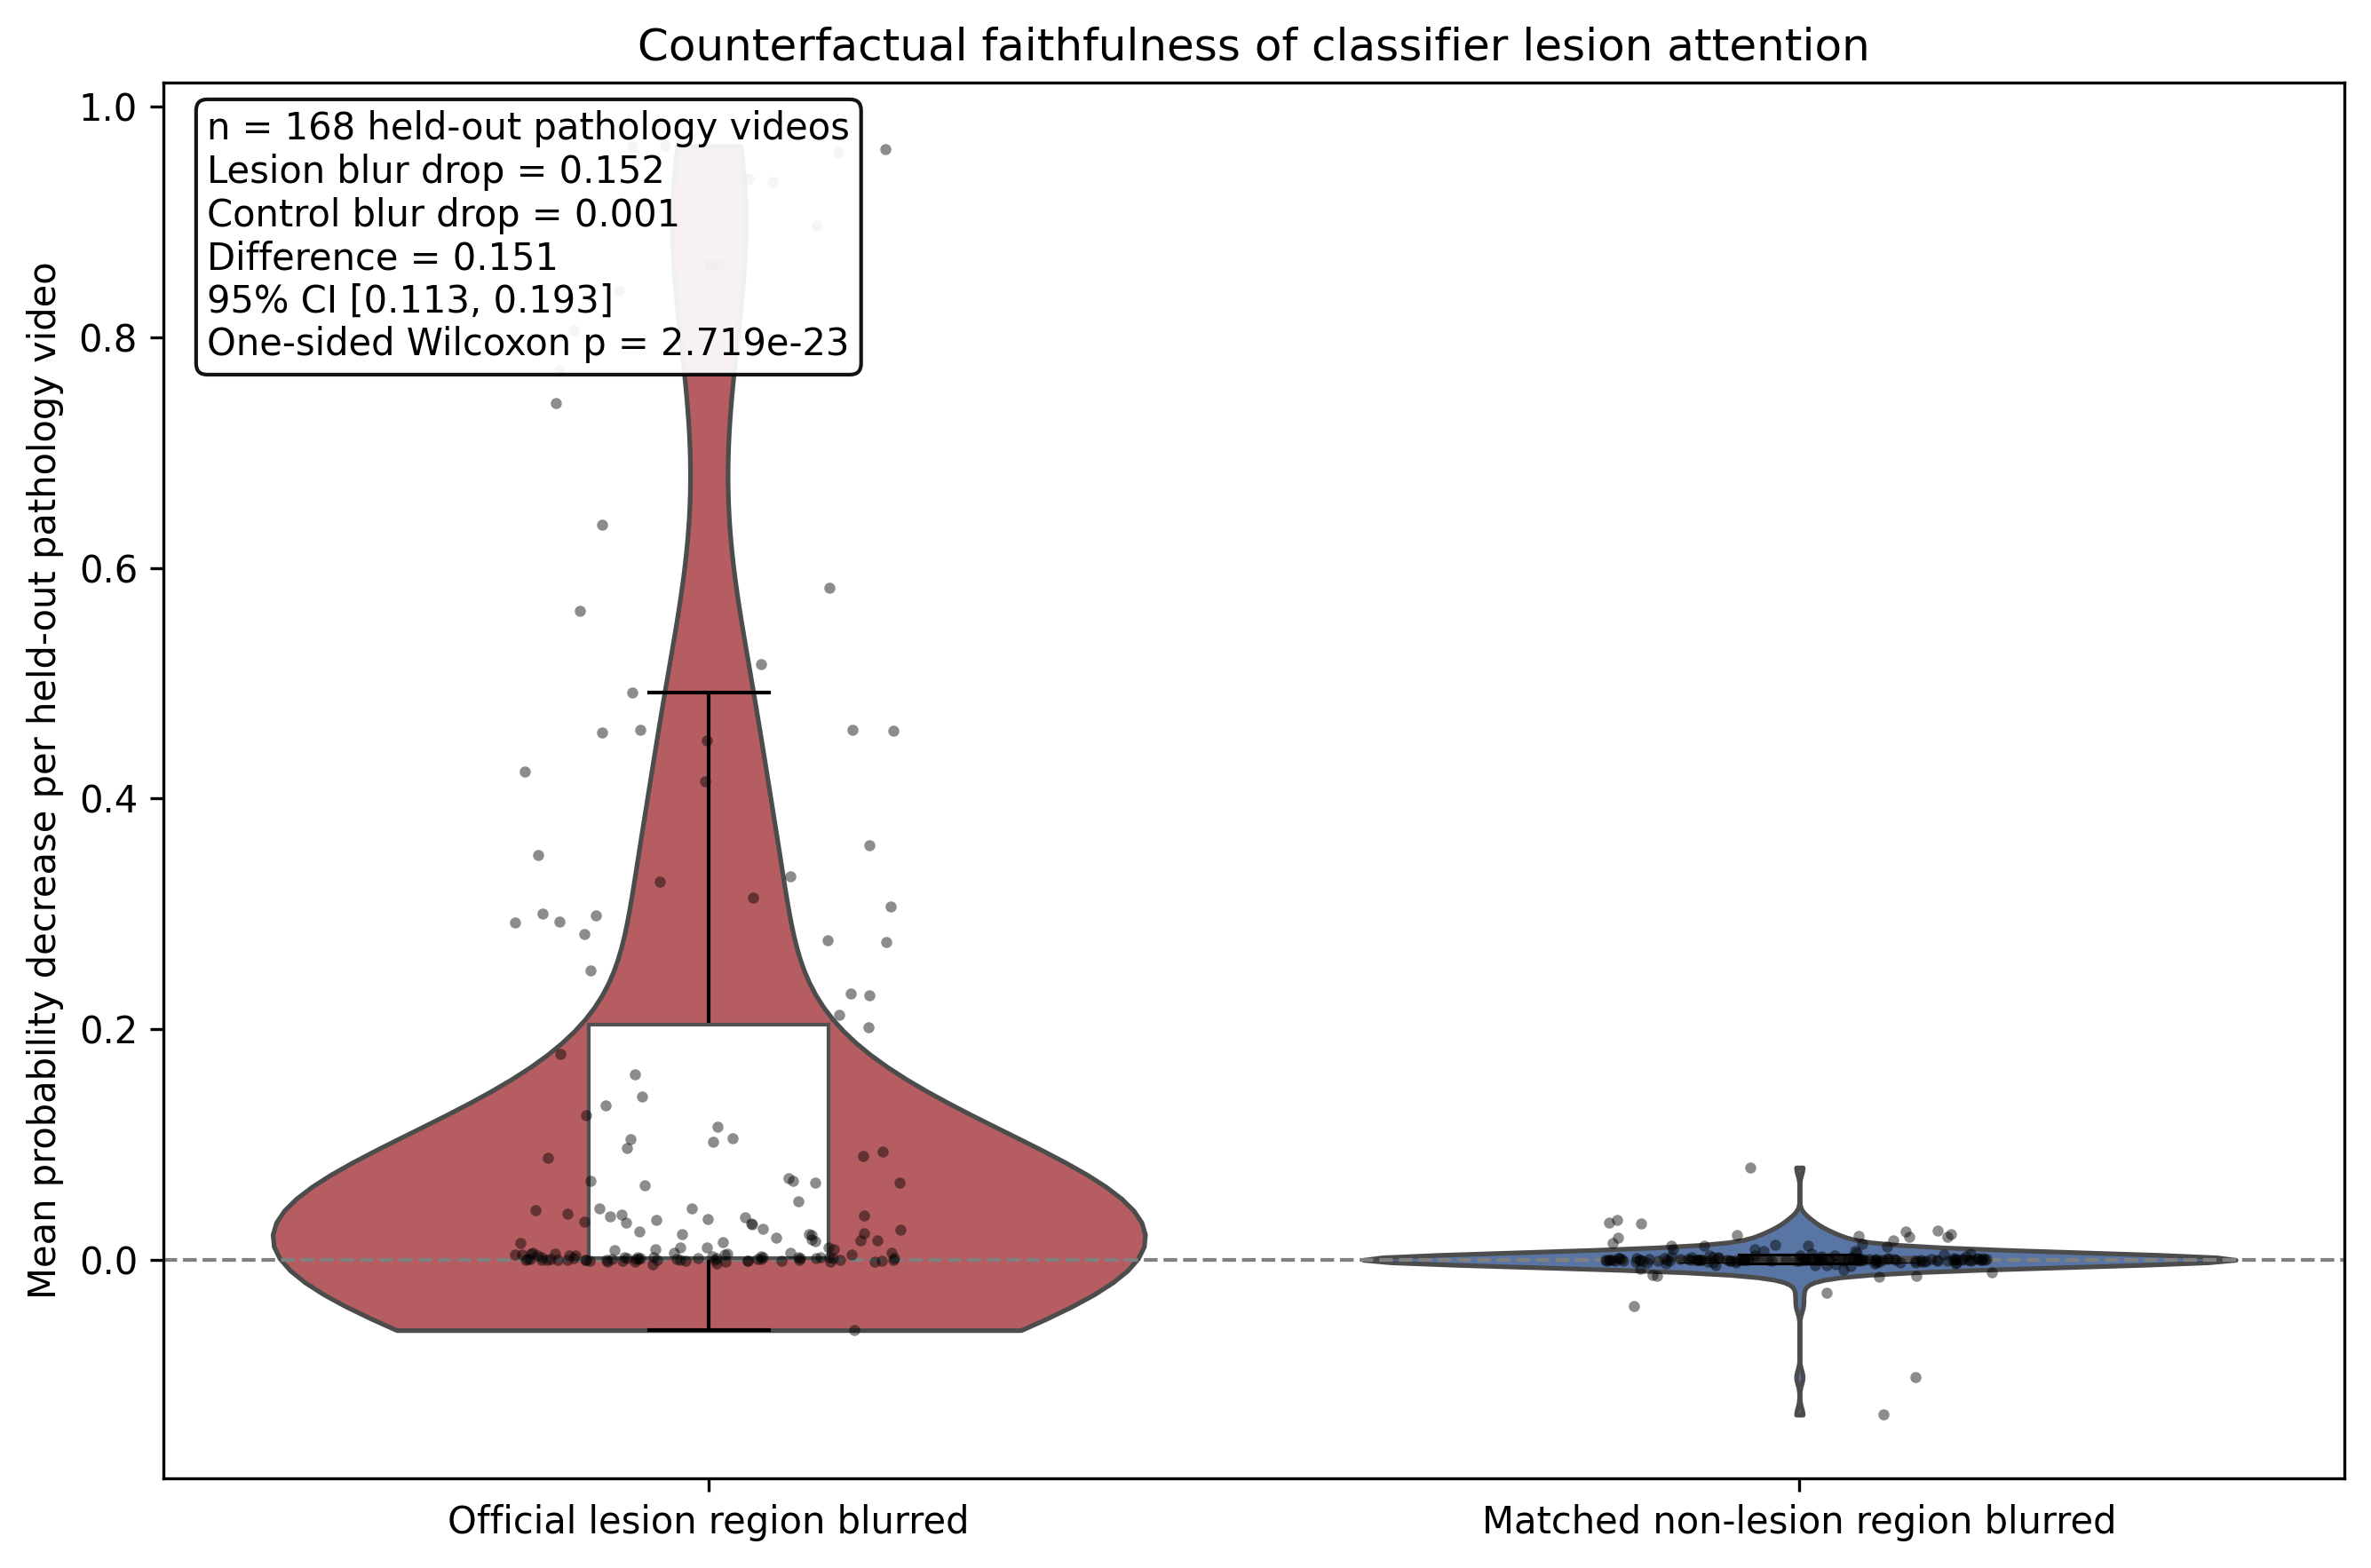
\includegraphics[width=0.96\columnwidth]{figure_gradcam_counterfactual_faithfulness.png}
\caption{Counterfactual faithfulness evaluation. Classifier confidence decreases far more after perturbing official lesion pixels than after perturbing matched non-lesion pixels.}
\label{fig:faithfulness}
\end{figure}

\section{Challenges and Practical Considerations}

\subsection{Small Dataset and Grouped Data Leakage}

A primary challenge was balancing rigorous validation against a small pathology dataset. Neighboring video frames may be highly correlated, but excluding entire videos from training decreases the quantity and visual diversity of available training data.

We addressed this by using grouped video-level folds. This choice may produce lower scores than random image-level cross-validation, but it reduces a major source of leakage. It also aligns more closely with the intended question: whether a model can generalize to unseen laparoscopic videos.

\subsection{Foreground Sparsity and Annotation Complexity}

Lesions frequently occupy a small part of an image. In addition, one frame may contain multiple source annotations. This creates severe foreground-background imbalance and makes conventional pixel accuracy uninformative.

We merged official source masks into canonical binary targets, used weighted BCE to increase the contribution of lesion pixels, and combined it with Dice loss to optimize overlap directly. Despite these mitigations, segmentation remained moderate and produced false positives, demonstrating the difficulty of the task.

\subsection{Compute Constraints and Training Reproducibility}

The project was developed in Google Colab, where GPU access was not always available and runtime disconnections could interrupt training. Large 3D or extended training approaches were not practical for the available environment.

We therefore used ImageNet pretrained models, modest epoch limits, early stopping, checkpoint saving after each epoch, persistent experiment histories, and local image caching. These decisions made the workflow feasible on CPU when necessary and ensured completed work was not lost after a connection interruption.

\subsection{Meaningful Explainability}

A further challenge was avoiding superficial XAI. Grad-CAM heatmaps are easy to generate but can be misleading if presented without evaluation. Their limited resolution and dependence on threshold selection can produce unstable mask-overlap values.

We addressed this by evaluating explanations quantitatively against official masks, comparing them against direct U-Net segmentation, and adding a counterfactual faithfulness experiment. This does not eliminate all XAI limitations, but it provides a more defensible evidence chain than visual examples alone.

\section{Discussion}

\subsection{Meaning of the Classification Results}

The classifier's mean fold-level AUC of 0.965 indicates strong discrimination between selected pathology and no-pathology frames under video-level cross-validation. This is a promising result, particularly because every held-out image was evaluated by a model that did not train on its source video.

However, the pooled threshold-0.50 confusion matrix demonstrates that high AUC does not imply a perfect clinical operating point. Specificity was lower than sensitivity, and 61 no-pathology images were falsely flagged. This is acceptable only in the limited context of a research prototype intended to prompt human review.

\subsection{Meaning of the Segmentation Results}

The U-Net's mean Dice of 0.438 represents moderate lesion overlap. It shows that the model can often identify lesion regions but cannot yet be considered a reliable contouring system. The false-positive rate on no-pathology images is particularly important, because a misleading overlay could distract a surgeon or reviewer.

The segmentation model should therefore be considered a visual localization aid. Future work should investigate calibration, uncertainty maps, post-processing, lesion-size stratification, temporal consistency, and more advanced segmentation methods. A self-configuring baseline such as nnU-Net could also be considered when resources and data preparation permit \cite{isensee2021nnunet}.

\subsection{Why Direct Segmentation Outperformed Grad-CAM}

The comparison between U-Net and Grad-CAM is conceptually expected. U-Net is trained from pixel-level targets and optimized to reproduce lesion masks. Grad-CAM is generated from a classifier trained only with image-level labels. It highlights image regions that influence a class score, but it is not optimized to reproduce lesion boundaries.

The observed video-level Dice difference of 0.185 supports this distinction quantitatively. The result does not mean Grad-CAM is unhelpful. Grad-CAM can still reveal classifier evidence, identify suspicious regions, and expose potential spurious attention. Its role is complementary to segmentation rather than identical.

\subsection{Interpretation of Faithfulness Analysis}

The perturbation experiment supports lesion relevance because the classifier probability decreased much more after blurring the true lesion region than after blurring a matched non-lesion region. This result strengthens the interpretation of Grad-CAM and classifier confidence.

Nevertheless, faithfulness analysis must be discussed carefully. Perturbation can introduce artifacts, and a lesion region may include contextual tissue that is also relevant to the classifier. The test therefore does not prove causal medical understanding. It demonstrates a narrower but valuable fact: within the evaluated images, the classifier's pathology confidence is more sensitive to lesion-region disruption than to matched control disruption.

\subsection{Comparison with Prior Work}

Zhu and Elbattah reported stronger classifier and Grad-CAM performance on GLENDA \cite{zhu2025xai}. Our paper should state this clearly and should not claim a new best classifier. The contribution of the present work is its comparative and evaluative structure: direct segmentation versus Grad-CAM localization, video-level aggregation, counterfactual faithfulness, and transparent visual failure analysis.

This positioning is scientifically stronger than overstating small-dataset performance. A reliable paper contribution can be methodological: showing that direct segmentation is spatially more accurate than post-hoc attention and that explanation evaluation benefits from functional testing.

\subsection{Clinical Translation Limitations}

This work does not establish clinical deployment readiness. The dataset comprises selected annotated frames rather than prospectively collected consecutive surgical video, and no external hospital, surgeon, camera, or patient cohort was included. The evaluated task is frame-level visible pathology recognition rather than patient-level diagnosis. In addition, the segmentation model produces substantial false-positive regions, the Grad-CAM threshold was selected in a pilot fold, and no clinician-reader study was conducted to assess accuracy, review time, confidence, trust, or automation bias. These constraints mean that the reported findings should be interpreted as evidence of technical feasibility within the evaluated dataset rather than evidence for clinical effectiveness or safety.

Before clinical use, future research should undertake external and prospective validation, uncertainty and calibration analysis, temporal modeling, lesion-subtype analysis, and clinician-centered usability evaluation. Explanations should support expert review and clinical judgement rather than replace them.

\section{Conclusion}

This paper presented a leakage-aware, video-level cross-validated framework for laparoscopic endometriosis classification, direct lesion segmentation, and explainability evaluation. The ImageNet-pretrained EdgeNeXt-Small classifier achieved strong discrimination, with mean fold-level ROC-AUC of $0.965\pm0.011$. The U-Net achieved mean positive-image Dice of $0.438\pm0.049$ and provided more accurate lesion localization than classifier Grad-CAM at both image and video levels. These findings demonstrate that reliable image-level discrimination and meaningful spatial localization should be assessed as related but distinct capabilities.

The principal contribution of this study is not a claim of a new state-of-the-art classifier. Rather, it is a rigorous evaluation framework that compares direct pixel-supervised lesion segmentation with post-hoc classifier attention under the same leakage-safe video-level cross-validation protocol. Official-mask overlap, image-level and video-level analyses, qualitative examples that include difficult cases, false-positive reporting, and lesion-versus-control counterfactual perturbation together provide a substantially stronger basis for interpreting model behavior than visual heatmaps alone.

The results support direct segmentation as the clearer localization output for a future expert-review tool, because it is explicitly optimized using lesion masks and achieved materially greater overlap with official annotations than Grad-CAM. Grad-CAM nevertheless remains useful for inspecting classifier attention and for identifying image regions associated with a pathology prediction. The faithfulness analysis further supports the conclusion that official lesion regions make a meaningful contribution to classifier confidence within the evaluated dataset.

Despite these encouraging results, the system remains a research prototype. Translation to practice requires external validation across institutions, cameras, operators, and patient populations; prospective assessment using temporally continuous surgical video; calibration and uncertainty analysis; and clinician-centered studies of usability, trust, and safety. Within these limits, the study provides a transparent and reproducible foundation for future computer-assisted laparoscopic endometriosis research in which classification, localization, and explainability are evaluated together rather than in isolation.

\section*{Data Availability and Reproducibility}

The GLENDA dataset is publicly available for non-commercial scientific research subject to its licensing and citation conditions \cite{leibetseder2020glenda}. This project preserves fixed video-level split manifests, model checkpoints, training histories, out-of-fold predictions, segmentation metrics, Grad-CAM maps, counterfactual-faithfulness results, and final figures. These artifacts support reproducibility within the evaluated dataset setting.

% Print deferred figures before the declaration and reference material,
% without forcing the references onto a separate page.
\FloatBarrier
\section*{Declarations}

\noindent\textbf{Author Contributions:} Nancy A. Mohamed contributed to conceptualization, research design, methodology development, implementation of the experimental pipeline, model training, cross-validation experiments, formal analysis, visualization, interpretation of results, and preparation of the original manuscript draft. Doha W. Eid contributed to dataset preparation, annotation-mask processing, experimental validation, and manuscript review. Nada H. Helmy contributed to literature review, evaluation design, statistical-result verification, and manuscript review. Malak A. Gaber contributed to data quality control, qualitative-result review, figure preparation, and manuscript review. Myrna A. Badr contributed to experimental organization, results review, manuscript revision, and preparation of supporting research materials. Mai S. Mabrouk provided research supervision, methodological guidance, academic oversight, critical review of the study design and manuscript, and overall supervisory direction.

\vspace{0.4em}
\noindent\textbf{Funding:} This research received no external funding.

\vspace{0.4em}
\noindent\textbf{Data Availability:} The study used the publicly available GLENDA dataset. Access to the dataset is governed by the original dataset terms, licensing conditions, and citation requirements \cite{leibetseder2020glenda}.

\vspace{0.4em}
\noindent\textbf{Code Availability:} The code, fixed cross-validation manifests, trained-model checkpoints, and derived evaluation artifacts are available from the authors upon reasonable request, subject to the licensing conditions of the underlying GLENDA dataset.

\vspace{0.4em}
\noindent\textbf{Ethics Approval and Consent to Participate:} Not applicable. This study involved secondary analysis of publicly available, de-identified laparoscopic-image data. No new human participants were recruited, no clinical interventions were performed, and no identifiable personal data were collected by the authors.

\vspace{0.4em}
\noindent\textbf{Consent for Publication:} Not applicable. The manuscript does not contain identifiable information relating to individual participants.

\vspace{0.4em}
\noindent\textbf{Competing Interests:} The authors declare no competing interests.

\bibliographystyle{IEEEtran}
\bibliography{references}

\end{document}
